% This is a beamer template created by bingining in Oct 12, 2013.
\documentclass[xcolor={svgnames},compress]{beamer} 
\usepackage[UTF8]{ctex}
\usetheme{Copenhagen}
\usefonttheme{professionalfonts}
\useoutertheme[footline=authortitle,subsection=false]{miniframes}
\setbeamercovered{transparent}
\setbeamercolor{bgcyan}{fg=black,bg=cyan}
\setbeamercolor{bggreen}{fg=black,bg=green}
\setbeamercolor{bgred}{fg=black,bg=red}
\hypersetup{
    colorlinks=true,        % color link
    citecolor=blue,         % cite color
    linkcolor=blue,         % link color
    urlcolor=blue      
}
\addtobeamertemplate{headline}{\hypersetup{linkcolor=.}}{}
\addtobeamertemplate{footline}{\hypersetup{linkcolor=.}}{}

\makeatletter
%\setbeamercolor{section in head/foot}{fg=white}
\setbeamercolor{title in head/foot}{parent=subsection in head/foot}
\setbeamertemplate{footline}
{
    \leavevmode%
    \hbox{%
        \begin{beamercolorbox}[wd=.333333\paperwidth,ht=2.25ex,dp=1ex,center]{author in head/foot}%
            \usebeamerfont{author in head/foot}\insertshortauthor
        \end{beamercolorbox}%
        \begin{beamercolorbox}[wd=.333333\paperwidth,ht=2.25ex,dp=1ex,center]{title in head/foot}%
            \usebeamerfont{title in head/foot}\hypersetup{hidelinks}%
            \insertshorttitle
        \end{beamercolorbox}%
        \begin{beamercolorbox}[wd=.333333\paperwidth,ht=2.25ex,dp=1ex,right]{date in head/foot}%
            \usebeamerfont{date in head/foot}\insertshortdate{}\hspace*{2em}
            \insertframenumber{} / \inserttotalframenumber\hspace*{2ex} 
    \end{beamercolorbox}}%
    \vskip0pt%
}
\makeatother
\beamertemplatenavigationsymbolsempty 
\hypersetup{pdfpagemode=FullScreen} % full-screen when viewing the pdf
\AtBeginSection[]
{
    \begin{frame}<beamer>
        \frametitle{提纲}
        \tableofcontents[currentsection]
    \end{frame}
}
%show a plan before every section
% ajust the vspace on item
\let\olditem\item
\renewcommand{\item}{%
    \olditem\vspace{\fill}}    

\setlength{\tabcolsep}{1pt}
\renewcommand{\arraystretch}{1.3} 

\usepackage[cal=rsfs,scr=euler]{mathalfa}
\usepackage{tabularx}
\usepackage{graphicx} % include graphs
\usepackage{colortbl,amsmath,amssymb}
\usepackage{textpos} % add logo
\usepackage{tensor} % manipulate tensor
\usepackage[most]{tcolorbox} % equation array box
\usepackage{multirow}


%%%%%%%%%%%%%%%%%%%%%%%%%%%%%%%%%%%%%%%%%%%%%%%%%%%%%%%%%%%%%%%%%%%%%%
% newcommand % 
%%%%%%%%%%%%%%%%%%%%%%%%%%%%%%%%%%%%%%%%%%%%%%%%%%%%%%%%%%%%%%%%%%%%%%
\usepackage{tensor}     % manipulate tensors
\usepackage{graphicx}   % include figures
\graphicspath{{Img/}} %Setting the graphicspath 
%\usepackage{bm}         % \bm{<text>} Bold math symbols
\usepackage{xcolor}     % textcolor
%\usepackage{cancel}     % slashes in equtions
%\usepackage{ulem}     % underline of equations
\usepackage{amsmath}	% AMS Math Package
\usepackage{amsthm}	% Theorem Formatting
\usepackage{amssymb}
\usepackage{datetime}
\usepackage{graphicx}
\usepackage{color}
%\usepackage{verbatim}
\usepackage{float}
%\usepackage{bm}

\newcommand{\nc}{\newcommand*}
\nc{\newc}{\newcommand}
\nc{\bm}[1]{\mathbf{#1}}
\nc{\figurewidth}{3.2in}
\nc{\xbar}{\bar{x}}
\nc{\rhoeq}{\rho_{\rm{eq}}}
\nc{\zeq}{z_{\rm{eq}}}
\nc{\la}{\lambda}
\nc{\tla}{\tilde{\la}}
\nc{\dt}{\delta}
\nc{\Dt}{\Delta}
\nc{\vj}{\vec{j}}
\nc{\vl}{\vec{l}}
\nc{\hx}{\hat{x}}
\nc{\hy}{\hat{y}}
\nc{\bj}{\mathbf{j}}
\nc{\mJ}{\mathcal{J}}
\nc{\mP}{\mathcal{P}}
\nc{\ga}{\gamma}
\nc{\Msun}{M_\odot}
\nc{\app}{\approx}
\nc{\av}[1]{\langle #1 \rangle}
\nc{\eq}[1]{Eq.~\eqref{#1}}
\nc{\al}{\alpha}
\nc{\Xstar}{X_{\ast}}
\nc{\seq}{\sigma_{\rm{eq}}}
\nc{\fpbh}{f_{\mathrm{PBH}}}
\nc{\VT}{\langle VT \rangle}


\nc{\s}{\sigma}
\nc{\Ld}{\Lambda}
\nc{\p}{\partial}
\nc{\Om}{\Omega}
\nc{\rd}{\mathrm{d}}
\nc{\Od}{\mathcal{O}}

%\nc{\ld}{\lambda}
%\nc{\gm}{\gamma}
\nc{\vth}{\vec{\theta}}
\nc{\vla}{\vec{\lambda}}
\nc{\vd}{\vec{d}}
\nc{\Mmin}{M_{\mathrm{min}}}
\nc{\rmd}{\mathrm{d}}
\nc{\mmin}{{m_{\mathrm{min}}}}
\nc{\mmax}{{m_{\mathrm{max}}}}
\nc{\mR}{\mathcal{R}}
\nc{\tmR}{\tilde{\mathcal{R}}}
\nc{\ogw}{\Omega_{\mathrm{GW}}}
\nc{\addref}{[\textcolor{red}{add ref}] }
\nc{\gpcyr}{\mathrm{Gpc}^{-3}\,\mathrm{yr}^{-1}}
\nc{\Eq}[1]{公式\eqref{#1}}
\nc{\Fig}[1]{图\ref{#1}}
\nc{\Table}[1]{表\ref{#1}}
\nc{\lvc}{LIGO-Virgo} % LIGO-VIRGO collaboration
\nc{\Sec}[1]{Sec.~\ref{#1}}
\nc{\eg}{\textit{e.g.~}}
\nc{\SNR}{\mathrm{SNR}}
\nc{\fpbhn}{f_{\mathrm{PBH0}}}    % f_pbh
\nc{\fmin}{{f_{\mathrm{min}}}}
\nc{\rhoGW}{\rho_{\mathrm{GW}}}
\nc{\Nobs}{N_{\mathrm{obs}}}
\nc{\km}{\mathrm{km}}
\nc{\Mpc}{\mathrm{Mpc}}
\nc{\Tobs}{T_{\mathrm{obs}}}
\nc{\Ntemp}{N_{\mathrm{temp}}}

\nc{\mH}{\mathcal{H}}
\nc{\cs}{c_s^2}
\nc{\Sij}[1]{S_{ij}^{(#1)}}
\nc{\vi}[1]{v_i^{(#1)}}
\nc{\no}{\nonumber}
\def\<{\left\langle}
\def\>{\right\rangle}
\def\ap{\alpha}
\def\half{{1\over 2}}
\nc{\bk}{\bm{k}}
\nc{\bq}{\bm{q}}
\nc{\bp}{\bm{p}}
\nc{\bl}{\bm{l}}
\nc{\bx}{\bm{x}}
\nc{\be}{\mathbf{e}}
\nc{\mS}{\mathcal{S}}
\nc{\te}{\tilde{\eta}}
\nc{\tp}{\tilde{p}}
\nc{\tk}{\tilde{k}}
\nc{\tx}{\tilde{x}}
\nc{\tF}{\tilde{F}}
\nc{\tA}{\tilde{A}}
\nc{\mkpq}{|\bk-\bp-\bq|}
\nc{\mpq}{|\bp-\bq|}
\nc{\mkp}{|\bk-\bp|}
\nc{\mSi}[1]{\mS^{(#1)}({\bk, \eta})}
\nc{\vk}{\vec{k}}
\nc{\kstar}{k_*}
\nc{\fstar}{f_*}
\nc{\xstar}{x_*}
\nc{\mpbh}{m_{\rm{pbh}}}
\nc{\bn}[1]{\dt\bm{t}_{\text{#1}}}
\nc{\bC}[1]{\bm{C}_{\text{#1}}}
\nc{\NTOA}{N_{\text{TOA}}}
\nc{\Nmode}{{N_{\text{mode}}}}
\nc{\ARN}{A_{\rm{RN}}}
\nc{\gRN}{\gamma_{\rm{RN}}}
\nc{\bS}{\mathbf{\Sigma}}
\nc{\br}{\mathbf{r}}
\nc{\bN}{\mathbf{R}}
\nc{\TTT}{\mathrm{TT}}

%%%%%%%%%%%%%%%%%%%%%%%%%%% greek letters %%%%%%%%%%%%%%%%%%%%%%%%%%%%
\newc{\zt}{\zeta}
\newc{\et}{\eta}
\newc{\ta}{\theta}
\newc{\io}{\iota}
\newc{\kp}{\kappa}
\newc{\La}{\Lambda}
\newc{\oo}{\omicron}
\newc{\sg}{\sigma}
\newc{\Sg}{\Sigma}
\newc{\om}{\omega}
\newc{\vp}{\varphi}
\newc{\Ga}{\Gamma}

%%%%%%%%%%%%%%%%%%%%%%%%%%%%%%% fonts %%%%%%%%%%%%%%%%%%%%%%%%%%%%%%%%
\newc{\mc}{\mathcal}
\newc{\ms}{\mathscr}
\newc{\mb}{\mathbf} 
\newc{\ie}{\textit{i.e. }}
\newc{\etc}{\textit{etc. }}
\newc{\etal}{\textit{et al. }}
\newc{\lcdm}{$\Lambda$CDM}
\newc{\gs}{\sqrt{-g}}

%%%%%%%%%%%%%%%%%%%%%%%%%%%%% other %%%%%%%%%%%%%%%%%%%%%%%%%%%%%%%%%%
\newc{\ts}{\tensor}
\newc{\td}{\tilde}
\newc{\hf}{\frac{1}{2}}
\newc{\ra}{\rightarrow}
\newc{\Ra}{\Rightarrow}
\newc{\lra}{\leftrightarrow}
\newc{\Lra}{\Leftrightarrow}
\newc{\so}{\therefore}
\newc{\nb}{\nabla}
\newc{\LA}{\mathop{}\!\mathbin\bigtriangleup} %Laplace
\newc{\DA}{\mathop{}\!\mathbin\Box} %DAlambert
\newc{\lp}{\left(} % left parenthesis
\newc{\rp}{\right)} % right parenthesis
\newc{\lb}{\left[} % left bracket
\newc{\rb}{\right]} % right bracket
\newc{\lB}{\left\{} % left Brace
\newc{\rB}{\right\}} % right Brace
\newc{\ef}{Eq.\eqref}
\newc{\red}[1]{\textcolor{red}{#1}}
\newc{\add}{\red{\emph{(add some comments or explanations)}\\}}
%%%%%%%%%%%%%%%%%%%%%% only used in this file %%%%%%%%%%%%%%%%%%%%%%%%
\newc{\Td}[1]{ \ts{\dt}{#1} }
\newc{\Th}[1]{\ts{h}{#1}} % tesor h
\newc{\h}[1]{\ts{\bar{h}}{#1}} % trace-reverse tensor
\newc{\Tg}[1]{\ts{\ga}{#1}}
\newc{\TG}[1]{\ts{\Ga}{#1}} % tensor \Gamma
\newc{\Bg}{\bm{g}}
\newc{\Bf}{\bm{f}}
\newc{\BG}{\bm{\ga}}
\newc{\tr}[1]{\lb #1 \rb}
\newc{\gts}{ \sqrt{-\td{g}}}
\newc{\nt}[1]{\ts{\td{\nabla}}{#1}}
\newc{\da}{\td{\DA}}
\newc{\tn}{\td{\nb}}
\newc{\Gone}[1]{\overset{1}{\Ga}\ts{}{#1}} 
\newc{\Gtwo}[1]{\overset{2}{\Ga}\ts{}{#1}}
\newc{\Etwo}[1]{\overset{2}{G}\ts{}{#1}} % second order of Einstein tensor 
\newc{\Rone}[1]{\overset{1}{R}\ts{}{#1}} 
\newc{\Rtwo}[1]{\overset{2}{R}\ts{}{#1}} 
%\newc{\TT}{\overset{TT}{=}} 
\nc{\TT}{\mathrm{TT}}
\newc{\hone}[1]{\overset{1}{h}\ts{}{#1}} 
\newc{\htwo}[1]{\overset{2}{h}\ts{}{#1}} 
\newcommand{\order}[1]{\mathcal{O}\left(#1\right)}
\newcommand{\avg}[1]{\left \langle #1 \right \rangle}
\nc{\GW}{\mathrm{GW}}
%%%%%%%%%%%%%%%%%%%%%%%%%%%%%%%%%%%% other %%%%%%%%%%%%%%%%%%%%%%%%%%%%%%%%%%%%
\def\half{{1\over 2}}

\def\p{\partial}
\def\ap{\alpha'}
\def\({\left(}
\def\){\right)}
\def\Mpl{M_{\rm P}}


%%%%%%%%%%%%%%%%%%%%%%%%%%%%%%%%%%% equations %%%%%%%%%%%%%%%%%%%%%%%%%%%%%%%%%%
\def\({\left(}
\def\){\right)}
\def\e{\begin{equation}}
\def\q{\end{equation}}
\def\m{\begin{eqnarray}}
\def\n{\end{eqnarray}}
\nc{\blue}[1]{\textcolor{blue}{#1}}
\nc{\Refs}[1]{{\tiny{\textcolor{blue}{\textit{#1}}}}}
%%%%%%%%%%%%%%%%%%%%%%%%%%%%%%%%%%%%%%%%%%%%%%%%%%%%%%%%%%%%%%%%%%%%%%%%%%%%%%%%
%%%%%%%%%%%%%%%%%%%%%%%%%%%%%%%%%%%%%%%%%%%%%%%%%%%%%%%%%%%%%%%%%%%%%%


%%%%%%%%%%%%%%%%%%%%%%%%%%%%%%%%%%%%%%%%%%%%%%%%%%%%%%%%%%%%%%%%%%%%%%%%%%%%%%%%
\begin{document}

\kaishu

%%%%%%%%%%%%%%%%%%%%%%%%%%%%%%%%%%%%%%%%%%%%%%%%%%%%%%%%%%%%%%%%%%%%%%
% add logo on every frame
\addtobeamertemplate{frametitle}{}{%
    \begin{textblock*}{50mm}(0.98\textwidth,-8.5mm)
        
\includegraphics[height=7mm,width=7mm]{./pic/cas_logo}
    \end{textblock*}
}
%%%%%%%%%%%%%%%%%%%%%%%%%%%%%%%%%%%%%%%%%%%%%%%%%%%%%%%%%%%%%%%%%%%%%%
% title page 
%%%%%%%%%%%%%%%%%%%%%%%%%%%%%%%%%%%%%%%%%%%%%%%%%%%%%%%%%%%%%%%%%%%%%%
\title{通过引力波探测原初黑洞}
\author[陈祖成]{\Large 报告人:陈祖成
    \\ 导\quad 师: 黄庆国}

%\date{\today}
\date{2021年5月20日}

\institute{\large 中国科学院理论物理研究所}

\titlegraphic{

\includegraphics[width=0.7\columnwidth]{./pic/ucas_logo}\quad

\includegraphics[width=0.16\columnwidth]{./pic/itp_logo.jpg}
}

%%%%%%%%%%%%%%%%%%%%%%%%%%%%%%%%%%%%%%%%%%%%%%%%%%%%%%%%%%%%%%%%%%%%%%
\begin{frame}[plain]
\titlepage
\end{frame}


\begin{frame}{引力波相关文章}
    \vspace{-2mm}
    \begin{enumerate}
        \item \href{https://journals.aps.org/prd/abstract/10.1103/PhysRevD.100.081301}{Probing primordial-black-hole dark matter with scalar induced gravitational waves} \\
        Phys.Rev.D 100 (2019) 8, 081301\\
        Chen Yuan, \textbf{Zu-Cheng Chen}, Qing-Guo Huang    
        
        \item \href{https://link.springer.com/article/10.1007/s11433-019-9605-5}{Measuring the tilt of primordial gravitational-wave power spectrum from observations}\\
        Sci.China Phys.Mech.Astron. 62 (2019) 11, 110421\\
        Jun Li, \textbf{Zu-Cheng Chen}, Qing-Guo Huang
        
        \item \href{https://journals.aps.org/prd/abstract/10.1103/PhysRevD.101.043019}{Log-dependent slope of scalar induced gravitational waves in the infrared regions}\\
            Phys.Rev.D 101 (2020) 4, 043019\\ 
        Chen Yuan, \textbf{Zu-Cheng Chen}, Qing-Guo Huang    
          
        
    \end{enumerate} 
\end{frame}

%%%%%%%%%%%%%%%%%%%%%%%%%%%%%%%%%%%%%%%%%%%%%%%%%%%%%%%%%%%%%%%%%%%%%%%%%%%%%%%%
\begin{frame}{引力波相关文章}
    \begin{enumerate}   
        \setcounter{enumi}{3} 
        \item \href{https://link.springer.com/article/10.1007\%2Fs11467-019-0936-x}{Extraction of gravitational wave signals with optimized convolutional neural network}\\
        Front.Phys.(Beijing) 15 (2020) 1, 14601\\
        Hua-Mei Luo, Wenbin Lin, \textbf{Zu-Cheng Chen}, Qing-Guo Huang  
        
        \item \href{https://journals.aps.org/prd/abstract/10.1103/PhysRevD.101.063018}{Scalar induced gravitational waves in different gauges}\\
        Phys.Rev.D 101 (2020) 6, 063018\\
        Chen Yuan, \textbf{Zu-Cheng Chen}, Qing-Guo Huang
        
        \item \href{https://arxiv.org/abs/2101.06869}{Non-tensorial Gravitational Wave Background in NANOGrav 12.5-Year Data Set}\\ \href{https://arxiv.org/abs/2101.06869}{arXiv:2101.06869 [astro-ph.CO]}\\
        \textbf{Zu-Cheng Chen}, Chen Yuan, Qing-Guo Huang
        %
    \end{enumerate} 
\end{frame}
%%%%%%%%%%%%%%%%%%%%%%%%%%%%%%%%%%%%%%%%%%%%%%%%%%%%%%%%%%%%%%%%%%%%%%

%%%%%%%%%%%%%%%%%%%%%%%%%%%%%%%%%%%%%%%%%%%%%%%%%%%%%%%%%%%%%%%%%%%%%%
\begin{frame}{原初黑洞相关文章}
    \vspace{-2mm}
    \begin{enumerate}
        \item \href{https://iopscience.iop.org/article/10.3847/1538-4357/aad6e2}{Merger Rate Distribution of Primordial-Black-Hole Binaries}\\
        Astrophys.J. 864 (2018) 1, 61\\
        \textbf{Zu-Cheng Chen},Qing-Guo Huang
        
        \item \href{https://iopscience.iop.org/article/10.3847/1538-4357/aaf581}{Stochastic Gravitational-Wave Background from Binary Black Holes and Binary Neutron Stars and Implications for LISA}\\
        Astrophys.J. 871 (2019) 1, 97\\
        \textbf{Zu-Cheng Chen}, Fan Huang, Qing-Guo Huang
        
        \item \href{https://iopscience.iop.org/article/10.1088/1475-7516/2020/08/039}{Distinguishing Primordial Black Holes from Astrophysical Black Holes by Einstein Telescope and Cosmic Explorer}\\
        JCAP 08 (2020) 039\\
        \textbf{Zu-Cheng Chen},Qing-Guo Huang
        
        \item \href{https://journals.aps.org/prl/abstract/10.1103/PhysRevLett.124.251101}{Pulsar Timing Array Constraints on Primordial Black Holes with NANOGrav 11-Year Dataset}\\
        Phys.Rev.Lett. 124 (2020) 25, 251101\\    
        \textbf{Zu-Cheng Chen}, Chen Yuan, Qing-Guo Huang 
        
    \end{enumerate} 
\end{frame}
%%%%%%%%%%%%%%%%%%%%%%%%%%%%%%%%%%%%%%%%%%%%%%%%%%%%%%%%%%%%%%%%%%%%%%
% contents
%%%%%%%%%%%%%%%%%%%%%%%%%%%%%%%%%%%%%%%%%%%%%%%%%%%%%%%%%%%%%%%%%%%%%%
\begin{frame}{提纲}
    %    \setcounter{tocdepth}{1}
    \tableofcontents
\end{frame}

%%%%%%%%%%%%%%%%%%%%%%%%%%%%%%%%%%%%%%%%%%%%%%%%%%%%%%%%%%%%%%%%%%%%%%
\section{引言}
\subsection{}
%%%%%%%%%%%%%%%%%%%%%%%%%%%%%%%%%%%%%%%%%%%%%%%%%%%%%%%%%%%%%%%%%%%%%%
\begin{frame}{}
    \centering
    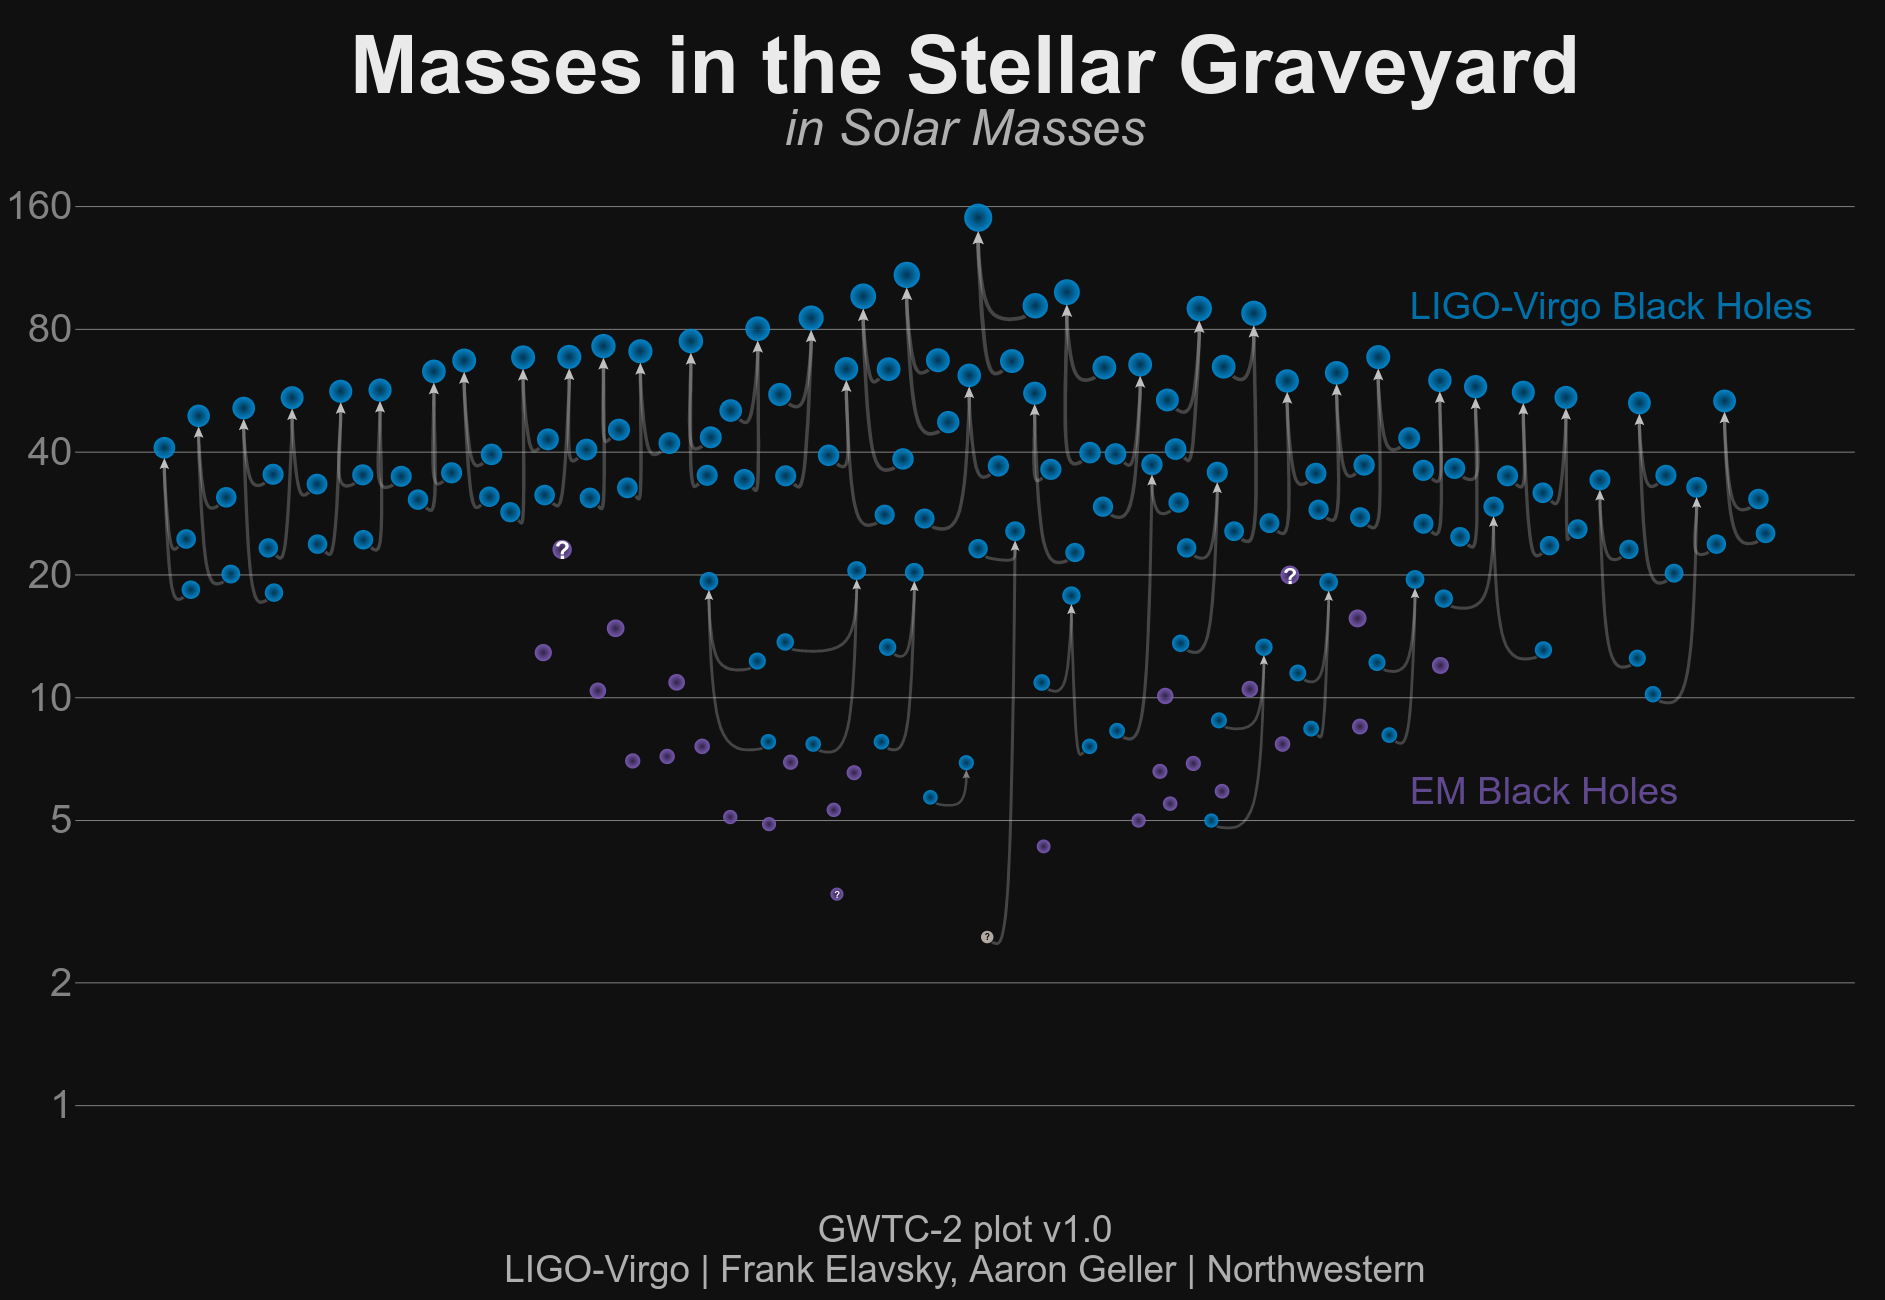
\includegraphics[width=\textwidth]{./pic/Masses_of_Dead_Stars_LIGO_Virgo}
\end{frame}
%%%%%%%%%%%%%%%%%%%%%%%%%%%%%%%%%%%%%%%%%%%%%%%%%%%%%%%%%%%%%%%%%%%%%%


%%%%%%%%%%%%%%%%%%%%%%%%%%%%%%%%%%%%%%%%%%%%%%%%%%%%%%%%%%%%%%%%%%%%%%
\begin{frame}{}
    \begin{block}{\lvc 的引力波探测告诉我们}
        \begin{itemize}
            \vspace{2mm}
            \item 宇宙中有很多双黑洞(BBH)。
            \item 这些双黑洞可以在哈勃时间内并合。
            \item 黑洞是有质量分布的。 
        \end{itemize}
    \end{block}
%    \pause
    \begin{alertblock}{未解之谜}
        \begin{itemize}
            \vspace{2mm}
            \item 这些黑洞的起源是什么?
            \item 以及是如何成对的?
            \item 为什么引力波探测到的黑洞的质量要比X射线探测到的黑洞的质量大很多?
        \end{itemize}
    \end{alertblock}
\centering
一个可能的解释是原初黑洞。
\end{frame}
%%%%%%%%%%%%%%%%%%%%%%%%%%%%%%%%%%%%%%%%%%%%%%%%%%%%%%%%%%%%%%%%%%%%%%


%%%%%%%%%%%%%%%%%%%%%%%%%%%%%%%%%%%%%%%%%%%%%%%%%%%%%%%%%%%%%%%%%%%%%%
\begin{frame}{原初黑洞(Primordial Black Hole, PBH)}
    \vspace{-3mm}
    \begin{columns}
        \begin{column}{0.7\textwidth}
            \begin{itemize}
                \item 原初黑洞是在宇宙早期由于原初密度扰动坍塌而形成的黑洞。
                \Refs{Mon.Not.Roy.Astron.Soc. 152 (1971) 75}
                \item 原初黑洞的质量可以跨越很多个数量级
                \e 
                m_{\mathrm{PBH}} \sim \frac{t}{G} \sim 10^{-18} 
                \left(
                \frac{t}{10^{-23}}
                \right) \Msun
                \q
                \item 未蒸发掉的原初黑洞可以作为暗物质的候选者。
                \item 原初黑洞可以解释\lvc 探测到的黑洞。
            \end{itemize}
        \end{column}
        \begin{column}{0.4\textwidth} 
            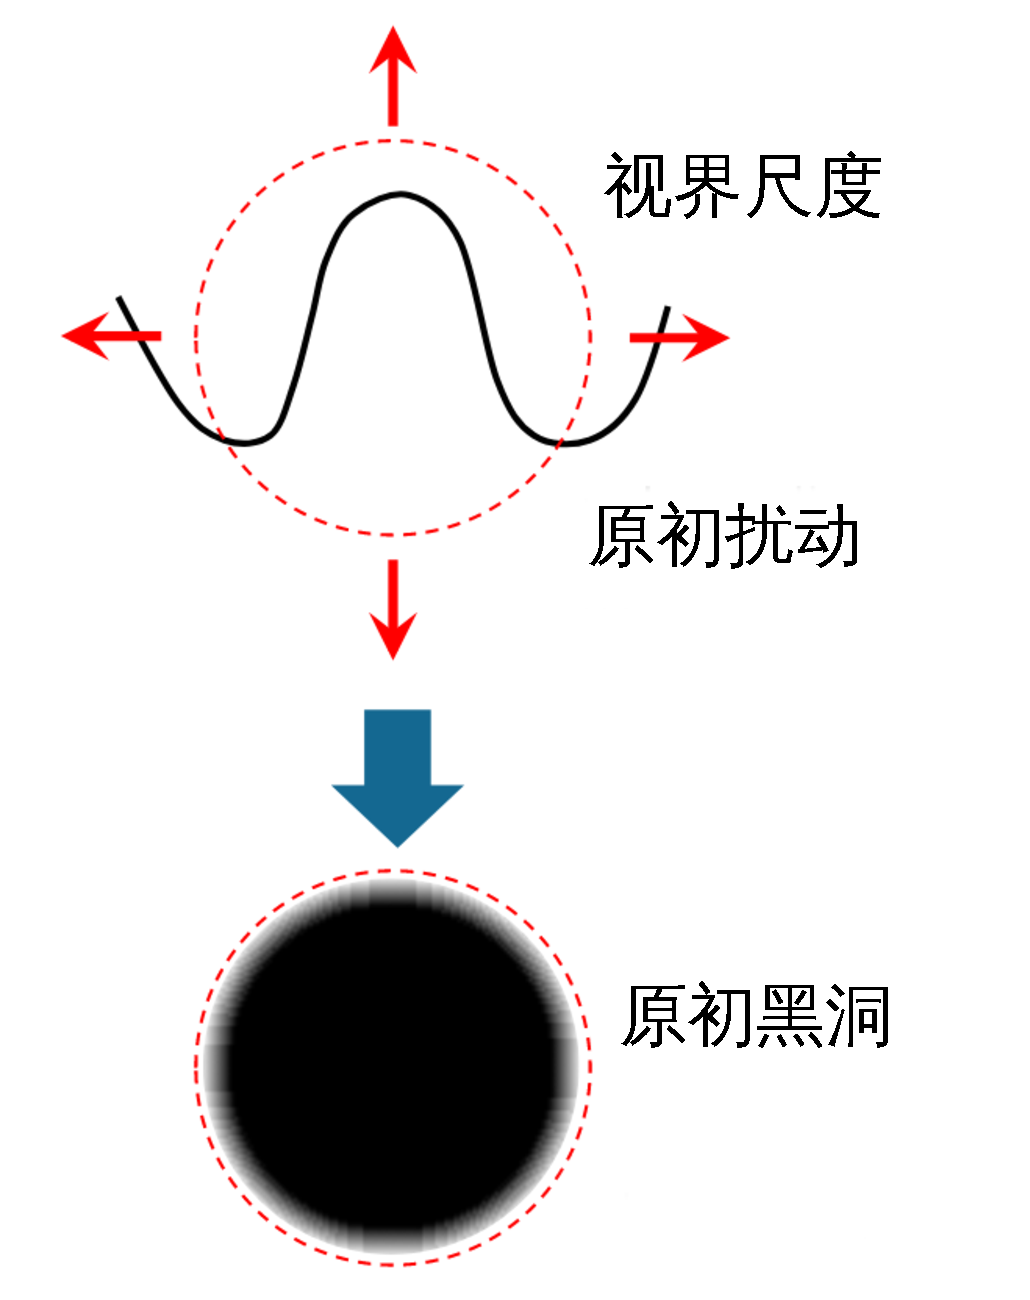
\includegraphics[width=\textwidth]{pic/pbh_form} 
        \end{column}
    \end{columns}
    \vspace{2mm}
%             
\end{frame}
%%%%%%%%%%%%%%%%%%%%%%%%%%%%%%%%%%%%%%%%%%%%%%%%%%%%%%%%%%%%%%%%%%%%%%

\section{原初双黑洞的并合率}
\subsection{}
%%%%%%%%%%%%%%%%%%%%%%%%%%%%%%%%%%%%%%%%%%%%%%%%%%%%%%%%%%%%%%%%%%%%%%
\begin{frame}{研究动机}
    \begin{itemize}
        \item 为了解释引力波探测到的双黑洞,需要知道原初双黑洞的并合率分布。
        \item 引力波探测到的黑洞是有质量分布的。
        \item 考虑任意的原初黑洞的质量谱$P(m)$
        {\small
        \[
        \int P(m)dm=1.
        \]
    }
        \centering
        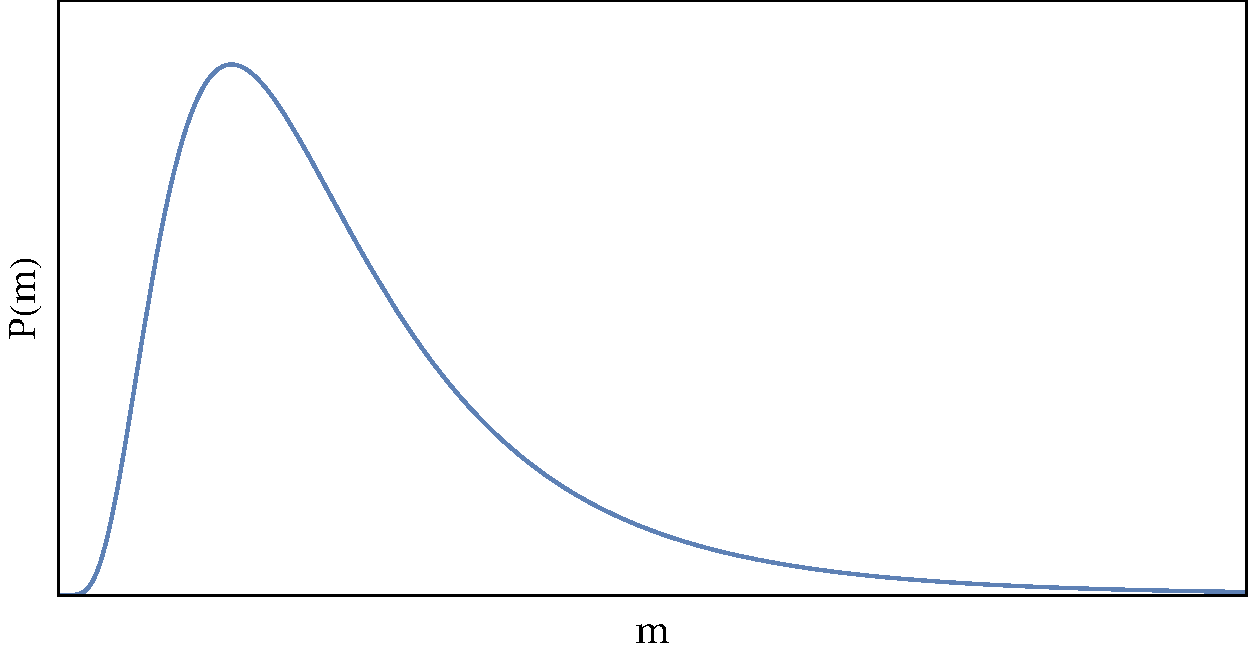
\includegraphics[width=0.7\textwidth]{pm} 
    \end{itemize}
\end{frame}
%%%%%%%%%%%%%%%%%%%%%%%%%%%%%%%%%%%%%%%%%%%%%%%%%%%%%%%%%%%%%%%%%%%%%%

%%%%%%%%%%%%%%%%%%%%%%%%%%%%%%%%%%%%%%%%%%%%%%%%%%%%%%%%%%%%%%%%%%%%%%
%%%%%%%%%%%%%%%%%%%%%%%%%%%%%%%%%%%%%%%%%%%%%%%%%%%%%%%%%%%%%%%%%%%%%%
\begin{frame}{原初双黑洞的形成}
    \vspace{-2mm}
    \begin{figure}[htbp!]
        \centering
        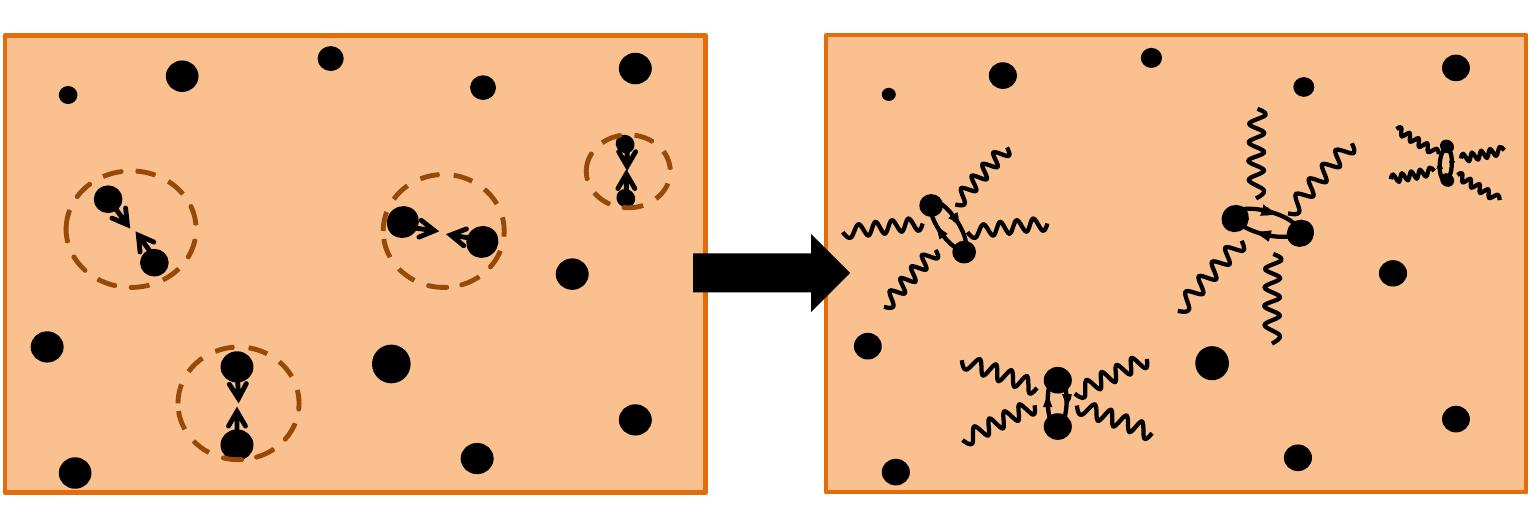
\includegraphics[width=\textwidth]{./pic/bbhs2.jpg}
    \end{figure}  \vspace{-2mm}
%    \hfill\Refs{Figure credit: CQG 35, 063001 (2018) \quad} 
    \begin{itemize}
        \item 在宇宙早期,原初黑洞是随机分布的。
        \item 最邻近的黑洞由于引力作用从宇宙膨胀背景中退耦出来。
        \item 其它原初黑洞和线性密度扰动提供初始角动量,进而形成有椭率的双黑洞系统。
        \item 由于引力辐射,原初双黑洞并合,并被\lvc 探测到。
    \end{itemize}
\end{frame}
%%%%%%%%%%%%%%%%%%%%%%%%%%%%%%%%%%%%%%%%%%%%%%%%%%%%%%%%%%%%%%%%%%%%%%
%%%%%%%%%%%%%%%%%%%%%%%%%%%%%%%%%%%%%%%%%%%%%%%%%%%%%%%%%%%%%%%%%%%%%%
\begin{frame}{原初双黑洞的动力学}
    \begin{itemize}       
        \vspace{-2mm}
        \item 运动方程
        \e\label{eom1}
        \ddot{r} - \( \dot{H} + H^2 \) r + \frac{m_b}{r^2} \frac{r}{|r|} = 0, \quad m_b = m_1 + m_2. 
        \q
        
        \item 双黑洞系统的半长轴$a$为
        \e
        a ={0.1 \xbar \over f_b} X^{\frac{4}{3}}, \quad X\equiv {x^3/\xbar^3}. 
        \label{axis}
        \q 
        \item 所有其他原初黑洞以及密度涨落产生的力矩 
        \e
        j_X\approx 0.5 \(f^2+\sigma_{\rm{eq}}^2\)^{1/2} {X\over f_b}. 
        \label{jx}
        \q
        \item 并合时间为 \Refs{Phys.Rev. 136 (1964) B1224-B1232}
        \m 
        t_c = \frac{3}{85} \frac{a^4}{m_i m_j m_b} j^7.
        \n 
        
    \end{itemize}
\end{frame}
%%%%%%%%%%%%%%%%%%%%%%%%%%%%%%%%%%%%%%%%%%%%%%%%%%%%%%%%%%%%%%%%%%%%%%
%%%%%%%%%%%%%%%%%%%%%%%%%%%%%%%%%%%%%%%%%%%%%%%%%%%%%%%%%%%%%%%%%%%%%%
\begin{frame}
    \frametitle{原初双黑洞并合率密度}
    
    \begin{tcolorbox}[ams align,colback=white!10!yellow]
        \mR_{12}(t) \approx&\, 3.9\cdot 10^6\times \red{\({t\over t_0}\)^{-{34\over 37}}} f^2 (f^2+\sigma_{\rm{eq}}^2)^{-{21\over 74}} \nonumber \\
        & \times  \min\(\frac{P(m_1)}{m_1}, \frac{P(m_2)}{m_2}\) \({P(m_1)\over m_1}+{P(m_2)\over m_2}\) \nonumber \\
        & \times (m_1 m_2)^{{3\over 37}} (m_1+m_2)^{36\over 37}\nonumber
    \end{tcolorbox}
    
    \begin{itemize}       
        \vspace{-2mm}
        \item 原初黑洞占冷暗物质的丰度$\red{f_{\rm{PBH}}\equiv \Omega_{\rm{PBH}}/\Omega_{\rm{CDM}}} \approx f/0.85$
        \item $\sigma_{\rm{eq}} \sim 0.005$是其它暗物质密度扰动的方差。
        \item 红移越大的时候,并合率越大$\Rightarrow$区分原初黑洞和天体物理黑洞
        
    \end{itemize}
\end{frame}
%%%%%%%%%%%%%%%%%%%%%%%%%%%%%%%%%%%%%%%%%%%%%%%%%%%%%%%%%%%%%%%%%%%%%%

%%%%%%%%%%%%%%%%%%%%%%%%%%%%%%%%%%%%%%%%%%%%%%%%%%%%%%%%%%%%%%%%%%%%%%
\begin{frame}{两种典型的质量谱}
    \vspace{-3mm}
    \begin{columns}
        \begin{column}{0.5\textwidth} 
            \begin{block}{幂率: $\al$}
                %             \vspace{-3mm}
                \[ 
                P(m)\approx {\alpha-1\over 5 \Msun} \({m\over 5 \Msun}\)^{-\alpha}
                \] 
                \vspace{-4.5mm}
            \end{block}  
        \end{column}
        \begin{column}{0.55\textwidth} 
            \begin{alertblock}{对数正态: $\s$, $m_c$}
                \[
                P(m) = \frac{1}{\sqrt{2 \pi} \sigma m} 
                e^{-\frac{\ln^2(m/m_c)}{2 \sigma^2}}
                \]
            \end{alertblock} 
        \end{column}
    \end{columns}
    \vspace{2mm}
    \centering
    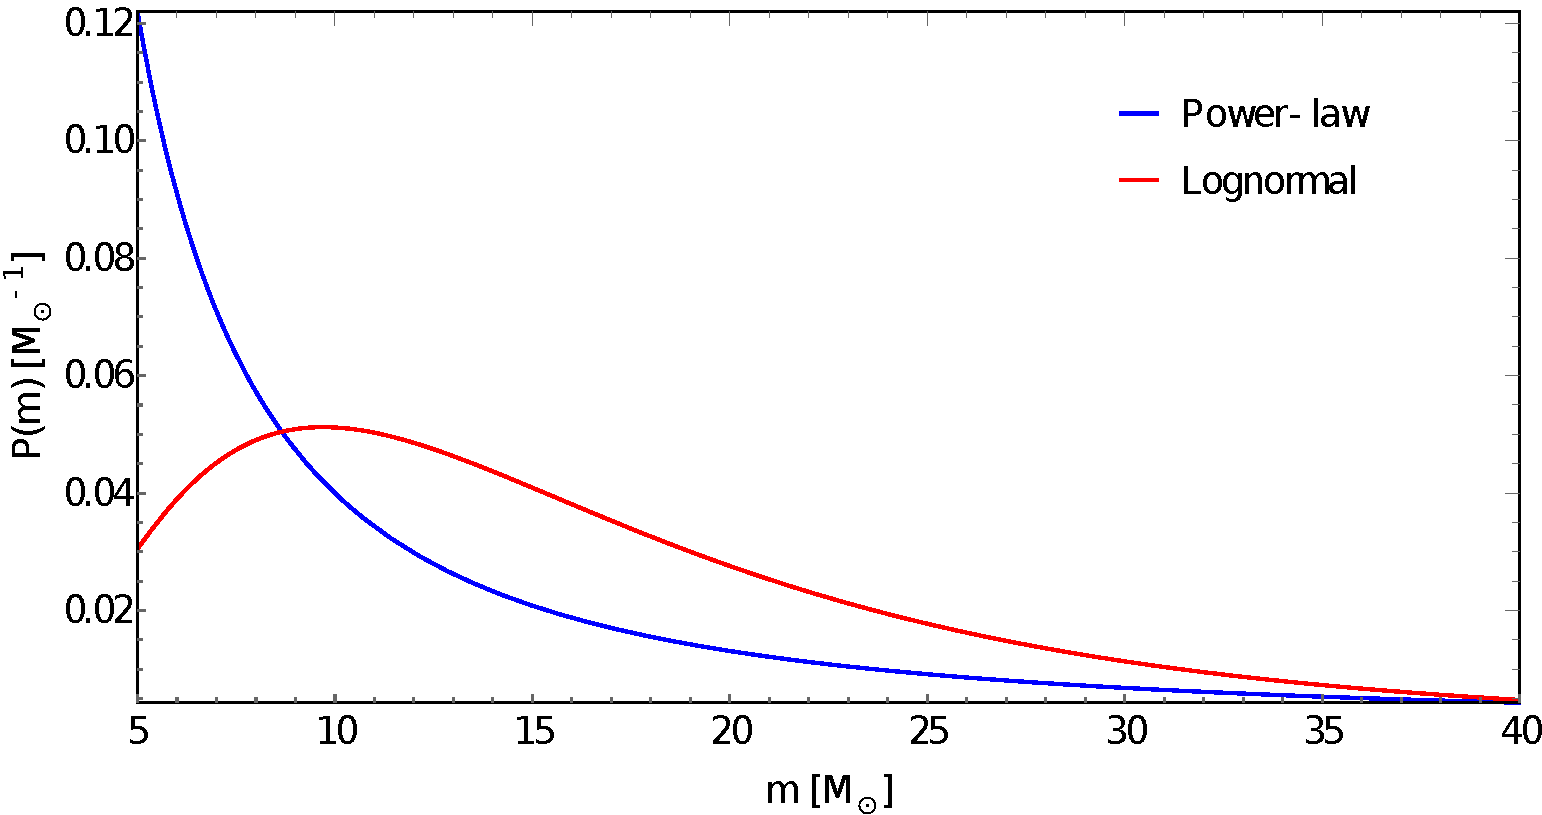
\includegraphics[width=0.9\textwidth]{pdfs}          
\end{frame}
%%%%%%%%%%%%%%%%%%%%%%%%%%%%%%%%%%%%%%%%%%%%%%%%%%%%%%%%%%%%%%%%%%%%%%

%%%%%%%%%%%%%%%%%%%%%%%%%%%%%%%%%%%%%%%%%%%%%%%%%%%%%%%%%%%%%%%%%%%%%
\begin{frame}
    \frametitle{引力波数据拟合}
    \begin{itemize}
        \item 我们需要从引力波数据中拟合出质量函数的参数$\vth$。
        \begin{itemize}
            \item 幂率: $\vth = \{\al\}$
            \item 对数正态: $\vth = \{m_c, \s\}$
        \end{itemize}
        
        \item 今天的并合率密度分布可以改写为
        \[ 
        \mR_{12}(t_0|\vth) = R\, p(m_1,m_2|\vth),
        \]
        \item 今天的并合率
        \[
        R = \int \mR_{12}(t_0|\vth)\ \rmd m_1\, \rmd m_2.
        \]
        
        \item 考虑的质量范围为$5\sim 100 \Msun$
    \end{itemize}
    
\end{frame}
%%%%%%%%%%%%%%%%%%%%%%%%%%%%%%%%%%%%%%%%%%%%%%%%%%%%%%%%%%%%%%%%%%%%%

%%%%%%%%%%%%%%%%%%%%%%%%%%%%%%%%%%%%%%%%%%%%%%%%%%%%%%%%%%%%%%%%%%%%%%
\begin{frame}{层次贝叶斯推断(Hierarchical Bayesian Inference)}
    \vspace{-7mm}
    \begin{equation*}\boxed{
            p(\vd|\vth, R) \propto R^{N} e^{-R\, \beta(\vth)} \prod_i^N 
            \int \rmd m_1 \rmd m_2\ p(d_i|m_1, m_2)\ p(m_1, m_2|\vth)
        }
    \end{equation*}
    
    \begin{itemize}
        \item $\vd = (d_1, \dots, d_N)$是探测到的$N$个引力波的数据。
        
        \item $\beta(\vth)$是平均的可探测时空体积
        \[ 
        \beta(\vth) \equiv \int \rmd m_1 \rmd m_2 \ VT(m_1, m_2)\ p(m_1, m_2|\vth)
        \]
        \item $p(d_i|m_1, m_2)$是单个引力波事件的似然函数
        \[
        p(d_i|m_1, m_2) \propto p(m_1, m_2|d_i)
        \]
    \end{itemize}	
    
\end{frame}
%%%%%%%%%%%%%%%%%%%%%%%%%%%%%%%%%%%%%%%%%%%%%%%%%%%%%%%%%%%%%%%%%%%%%%

%%%%%%%%%%%%%%%%%%%%%%%%%%%%%%%%%%%%%%%%%%%%%%%%%%%%%%%%%%%%%%%%%%%%%%
\begin{frame}
    \frametitle{使用LIGO O1的数据}
    \vspace{-3mm}
    \begin{columns}
        \begin{column}{0.5\textwidth} 
            \begin{figure}[htbp!]
                \centering
                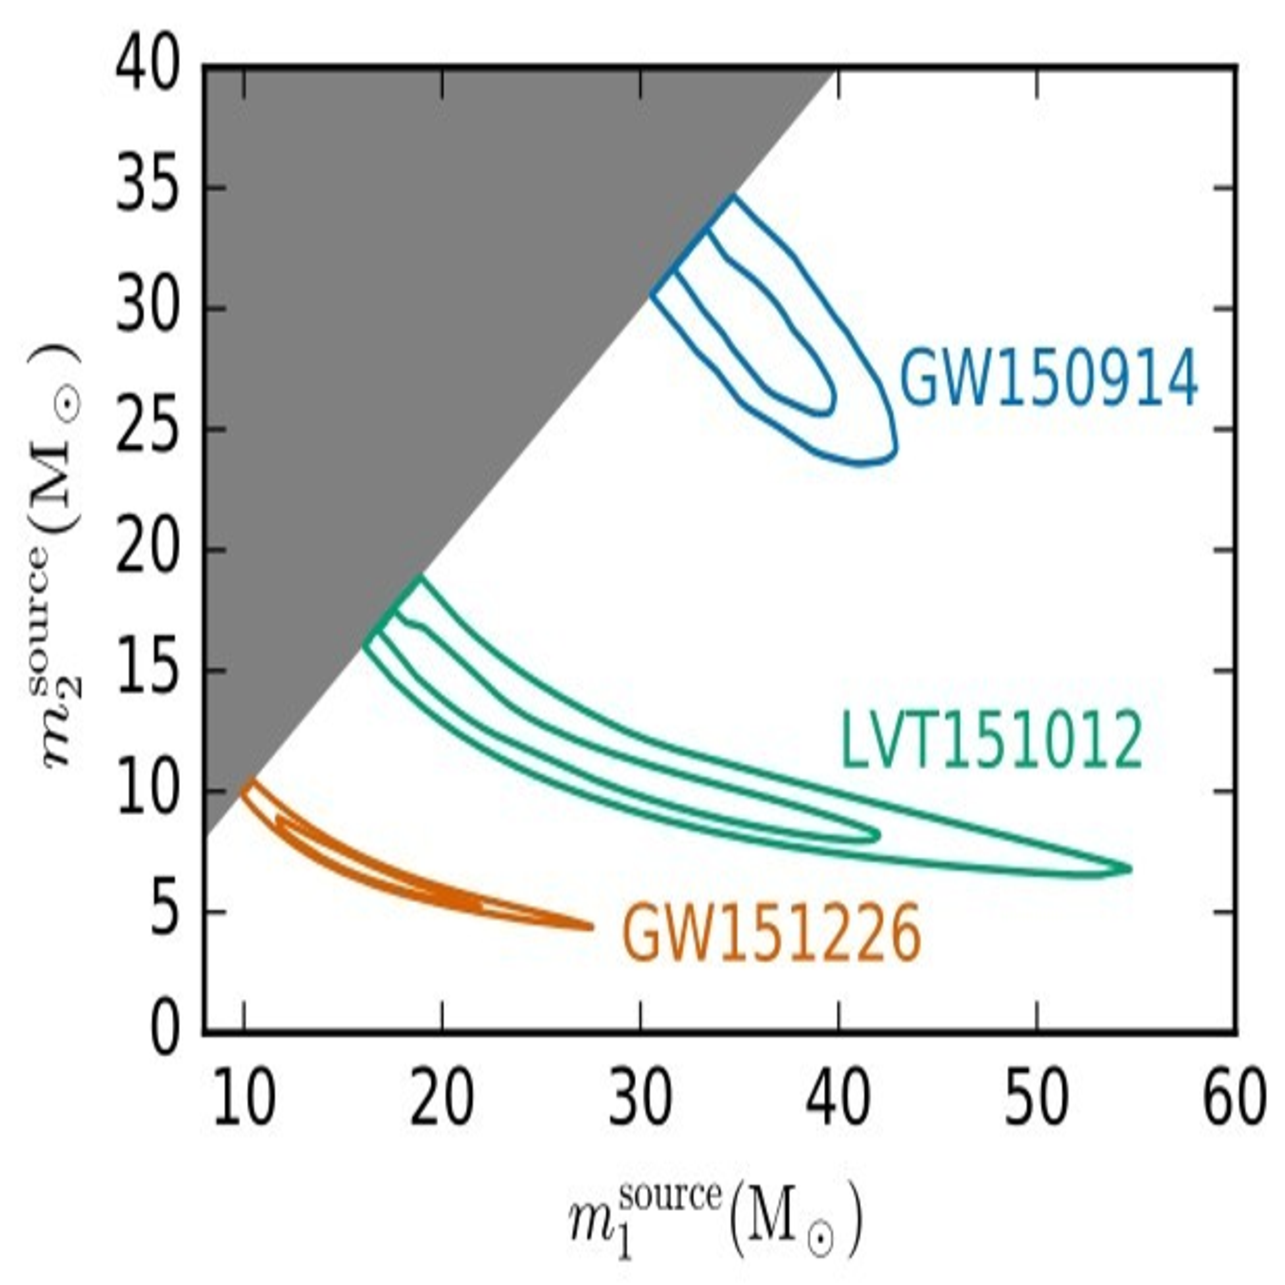
\includegraphics[width = \textwidth]{./pic/mass_post.pdf}
            \end{figure}
            \vspace{-3.mm}
            \centering
            后验分布 \textcolor{blue}{$p(m_1, m_2|d_i)$}
        \end{column}
        \begin{column}{0.58\textwidth} 
            \begin{figure}[htbp!]
                \centering
                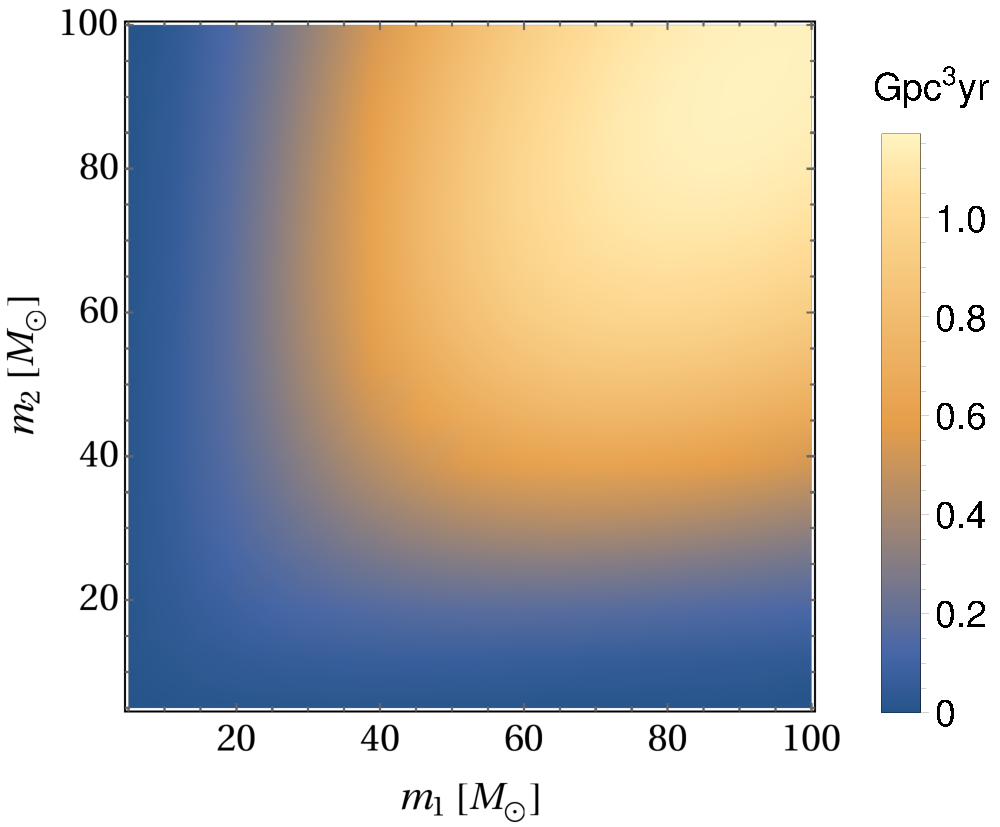
\includegraphics[width = \textwidth]{./pic/vt.pdf}
            \end{figure}			
            \vspace{-1.5mm}
            \centering
            时空体积 \textcolor{blue}{$VT(m_1,m_2)$}
        \end{column}
    \end{columns}
\end{frame}
%%%%%%%%%%%%%%%%%%%%%%%%%%%%%%%%%%%%%%%%%%%%%%%%%%%%%%%%%%%%%%%%%%%%%%
%%%%%%%%%%%%%%%%%%%%%%%%%%%%%%%%%%%%%%%%%%%%%%%%%%%%%%%%%%%%%%%%%%%%%%
\begin{frame}
    \frametitle{幂率: $P(m)\approx {\alpha-1\over 5\Msun} \({m\over 5\Msun}\)^{-\alpha}$}
    \begin{block}{}\small{
            %             \vspace{-3mm}
            \[ 
            \{\al,\, R,\, \fpbh\} = \{1.61,\ 80\,^{+108}_{-56} \gpcyr,\
            3.8\,^{+2.3}_{-1.8} \times 10^{-3}\}
            \] 
        }\vspace{-4mm} 
    \end{block} 
    \begin{figure}[htbp!]
        \centering
        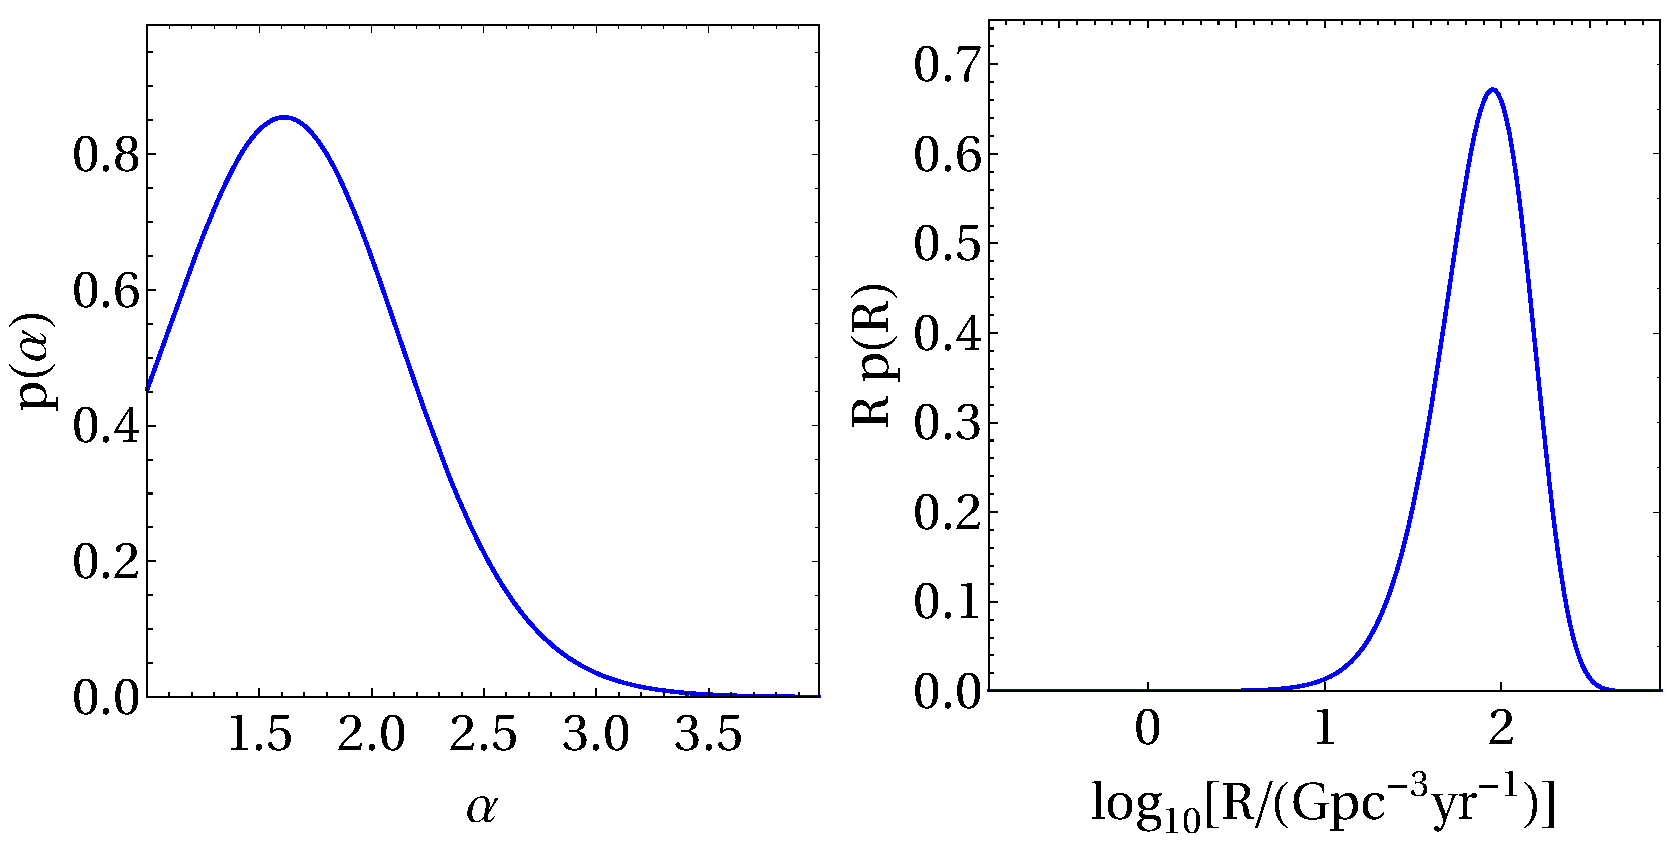
\includegraphics[width = \textwidth]{./pic/posterior-PBH-power.pdf}
    \end{figure}
\end{frame}
%%%%%%%%%%%%%%%%%%%%%%%%%%%%%%%%%%%%%%%%%%%%%%%%%%%%%%%%%%%%%%%%%%%%%%

%%%%%%%%%%%%%%%%%%%%%%%%%%%%%%%%%%%%%%%%%%%%%%%%%%%%%%%%%%%%%%%%%%%%%%
\begin{frame}
    \frametitle{对数正态: \large $P(m) = \frac{1}{\sqrt{2 \pi} \sigma m} 
        e^{-\frac{\ln^2(m/m_c)}{2 \sigma^2}}$ }
    \begin{block}{}\vspace{-3mm}\small{
            \[
            \{\s,\, m_c,\, R,\, \fpbh\} = \{0.65,\ 14.8 \Msun,\ 
            55\,^{+74}_{-38} \gpcyr,\ 2.8\,^{+1.6}_{-1.3} \times 10^{-3}\}
            \]
        }
        \vspace{-4mm}
    \end{block}  
    \begin{figure}[htbp!]
        \centering
        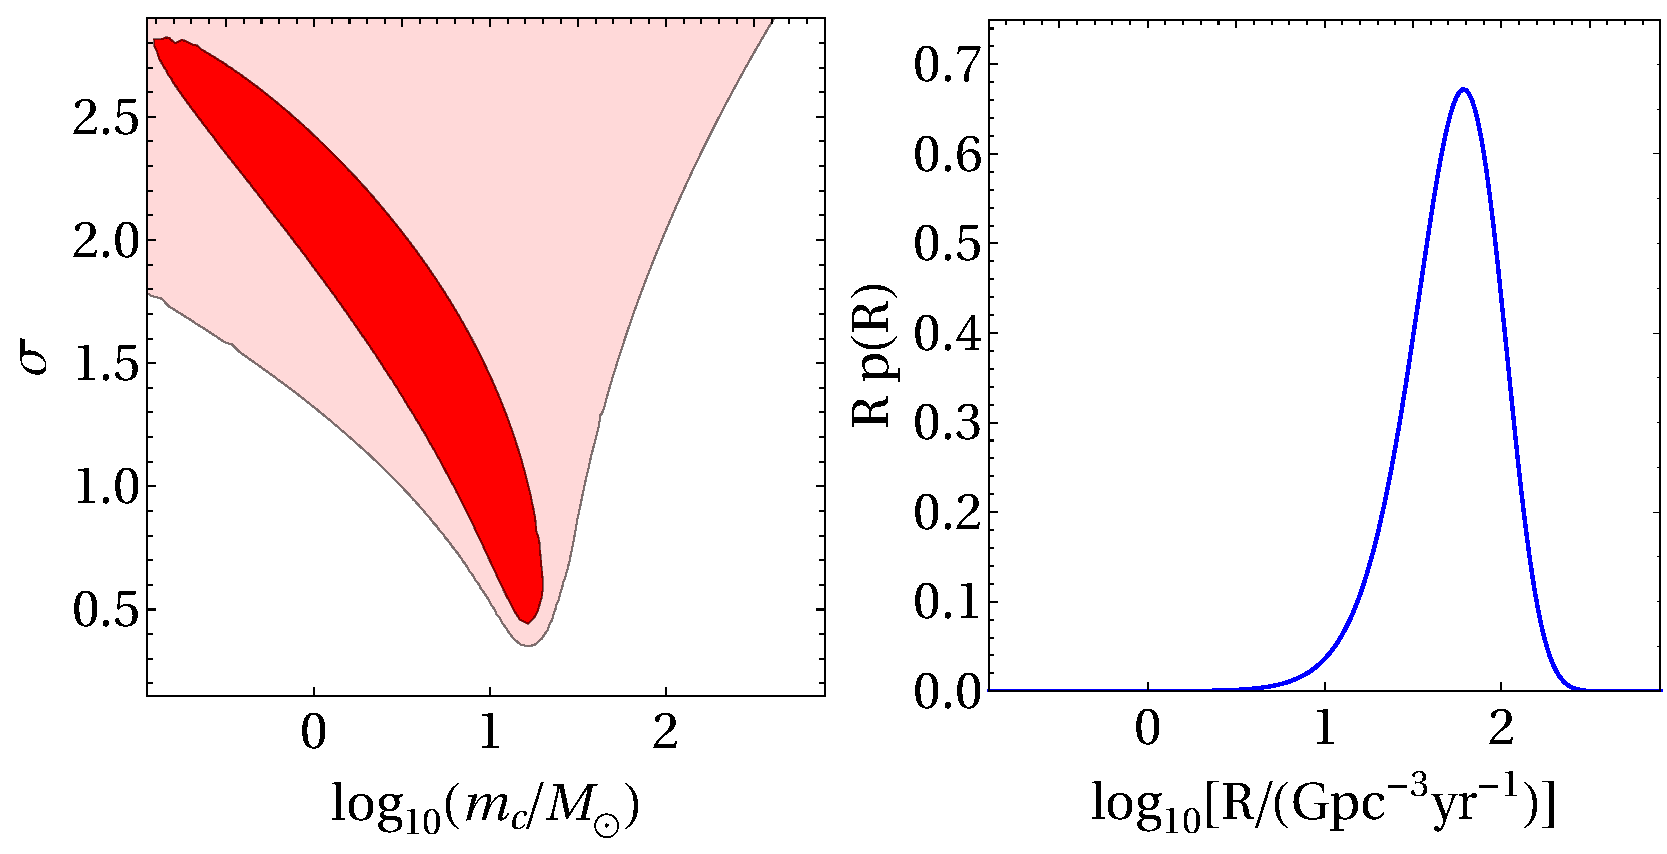
\includegraphics[width = \textwidth]{./pic/posterior-PBH-log.pdf}
    \end{figure}
\end{frame}
%%%%%%%%%%%%%%%%%%%%%%%%%%%%%%%%%%%%%%%%%%%%%%%%%%%%%%%%%%%%%%%%%%%%%%

%%%%%%%%%%%%%%%%%%%%%%%%%%%%%%%%%%%%%%%%%%%%%%%%%%%%%%%%%%%%%%%%%%%%%%
\begin{frame}
    \frametitle{二维的可探测事件数分布}	
    		\vspace{-2mm}
    \centering    
    用O1的结果来估算O2的可探测事件数
    \begin{columns}
        \begin{column}{0.56\textwidth} 
            \begin{figure}[htbp!]
                \centering
                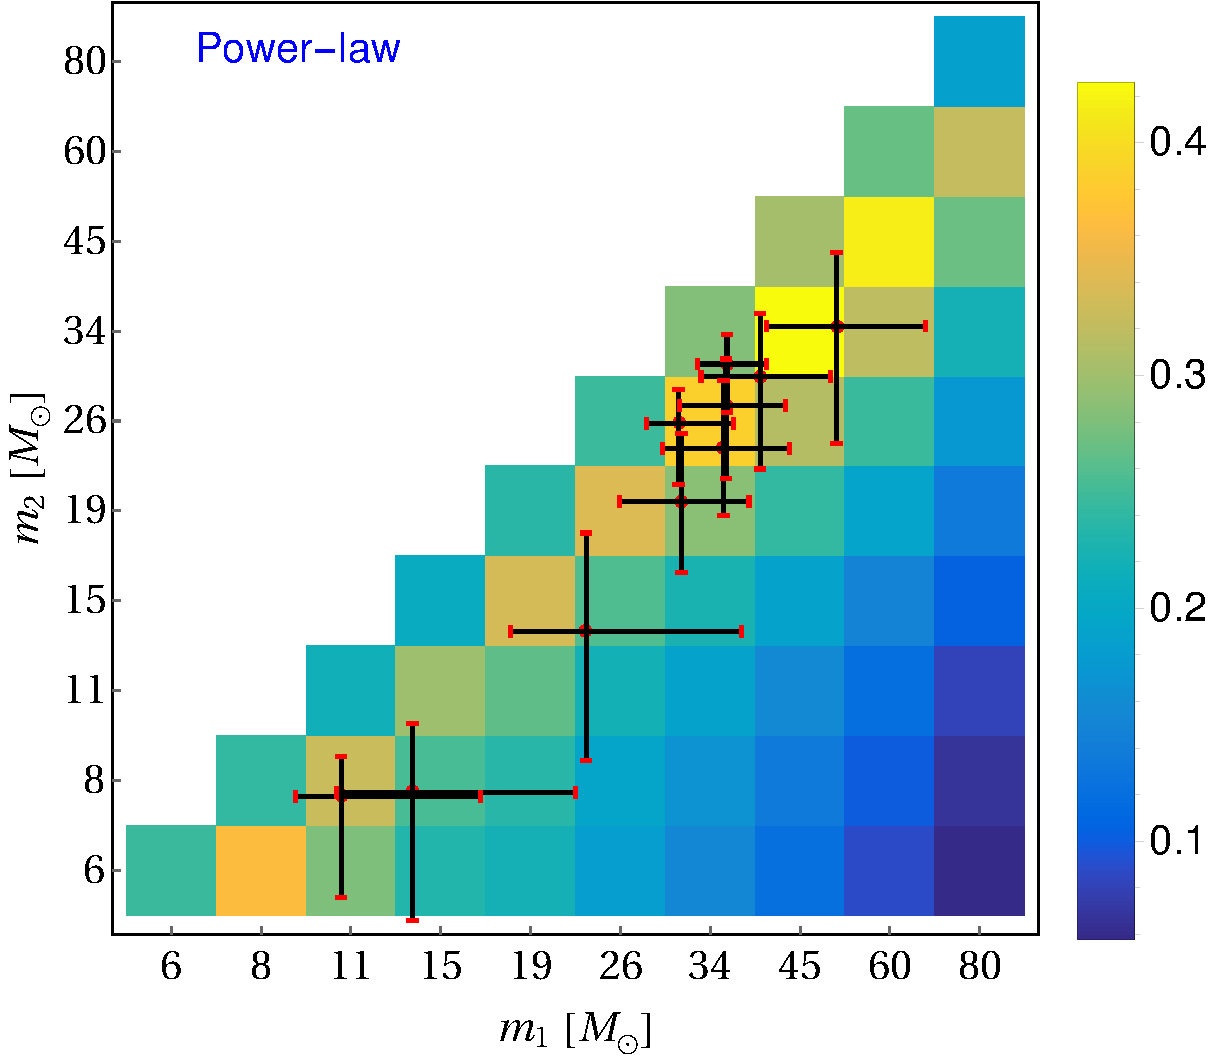
\includegraphics[width = \textwidth]{./pic/events_power01.pdf}
            \end{figure}
            \vspace{-3mm}
            \centering
            \red{$N_{\rm O1+O2} = 12^{+17}_{-9}$}
        \end{column}
        \begin{column}{0.56\textwidth} 
            \begin{figure}[htbp!]
                \centering
                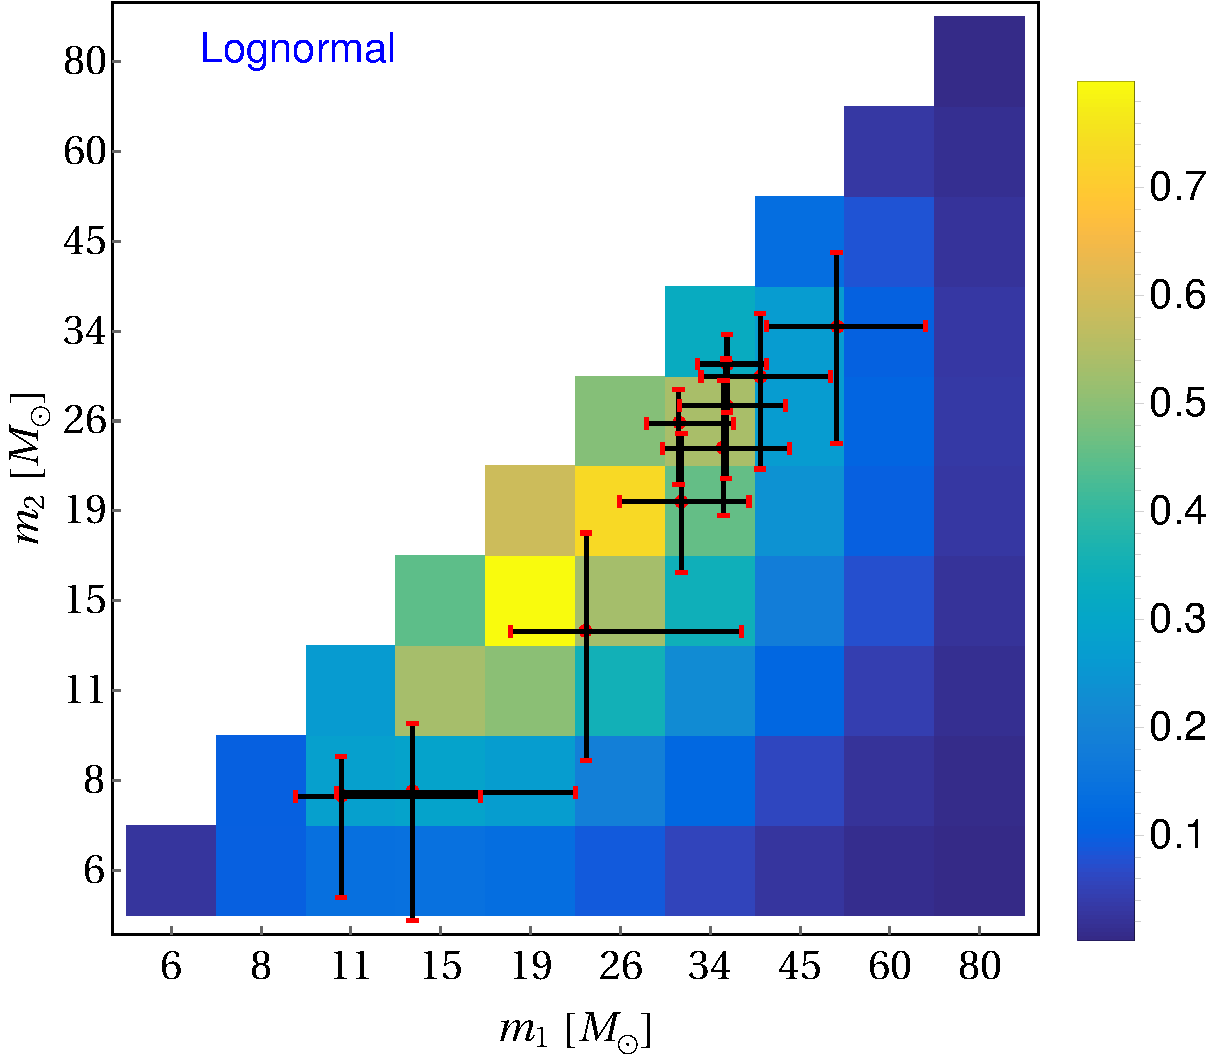
\includegraphics[width = \textwidth]{./pic/events_log01.pdf}
            \end{figure}
            \vspace{-3mm}
            \centering
            \red{$N_{\rm O1+O2} = 11^{+15}_{-8}$}
        \end{column}
    \end{columns}
\vspace{1mm}

\textcolor{blue}{随着引力波数据的积累,我们可以重构质量谱。}
\end{frame}
%%%%%%%%%%%%%%%%%%%%%%%%%%%%%%%%%%%%%%%%%%%%%%%%%%%%%%%%%%%%%%%%%%%%%%

%%%%%%%%%%%%%%%%%%%%%%%%%%%%%%%%%%%%%%%%%%%%%%%%%%%%%%%%%%%%%%%%%%%%%%
\begin{frame}{小结}	
    \begin{itemize}        
        \item 计算了原初黑洞具有一般质量谱时,原初双黑洞的并合率分布。
        \item 证实原初黑洞可以解释\lvc 探测到的双黑洞事件。
        \item 证实绝大多数的冷暗物质不是由恒星级质量的原初黑洞构成的。
    \end{itemize}
\end{frame}
%%%%%%%%%%%%%%%%%%%%%%%%%%%%%%%%%%%%%%%%%%%%%%%%%%%%%%%%%%%%%%%%%%%%%%

%%%%%%%%%%%%%%%%%%%%%%%%%%%%%%%%%%%%%%%%%%%%%%%%%%%%%%%%%%%%%%%%%%%%%%

\section{原初双黑洞产生的引力波背景}
\subsection{}
%%%%%%%%%%%%%%%%%%%%%%%%%%%%%%%%%%%%%%%%%%%%%%%%%%%%%%%%%%%%%%%%%%%%%%
\begin{frame}{研究动机}
    \begin{itemize}
        \item \lvc 目前只能探测到红移$z\lesssim 2$的双黑洞并合事件。
        \item 所有双黑洞并合产生的引力波信号会叠加形成随机引力波背景。
        \item 除了探测单个原初双黑洞产生的引力波外,还可以探测原初双黑洞产生的随机引力波背景。
    \end{itemize}
\end{frame}
%%%%%%%%%%%%%%%%%%%%%%%%%%%%%%%%%%%%%%%%%%%%%%%%%%%%%%%%%%%%%%%%%%%%%%

%%%%%%%%%%%%%%%%%%%%%%%%%%%%%%%%%%%%%%%%%%%%%%%%%%%%%%%%%%%%%%%%%%%%%%
\begin{frame}
    \frametitle{随机引力波背景 (SGWB)}
    \vspace{-2mm}
    %The energy-density spectrum of a GW background  is 
    %characterized by the dimensionless quantity
    %\[
    %   \ogw(\nu) = \frac{\nu}{\rho_c} \frac{d \rho_{\rm{GW}}}{d\nu},
    %\] 
    %which represents the  contribution of GW to the critical energy
    %density of the Universe, $\rho_c = 3H_0^2/(8\pi G)$,
    %and can be expressed as
    \begin{block}{}\vspace{-1mm}
        \[\small{
            \ogw(\nu) \equiv \frac{\nu}{\rho_c} \int dz\, dm_1\, dm_2 
            \frac{\mR_{12}(z)}{\(1+z\) H(z)} 
            \frac{dE_{\rm{GW}}}{d\nu_s}
        }
        \]
    \end{block}
    \vspace{-2mm}
    \begin{columns}
        \begin{column}{0.54\textwidth} 
            \begin{figure}[htbp!]
                \centering
                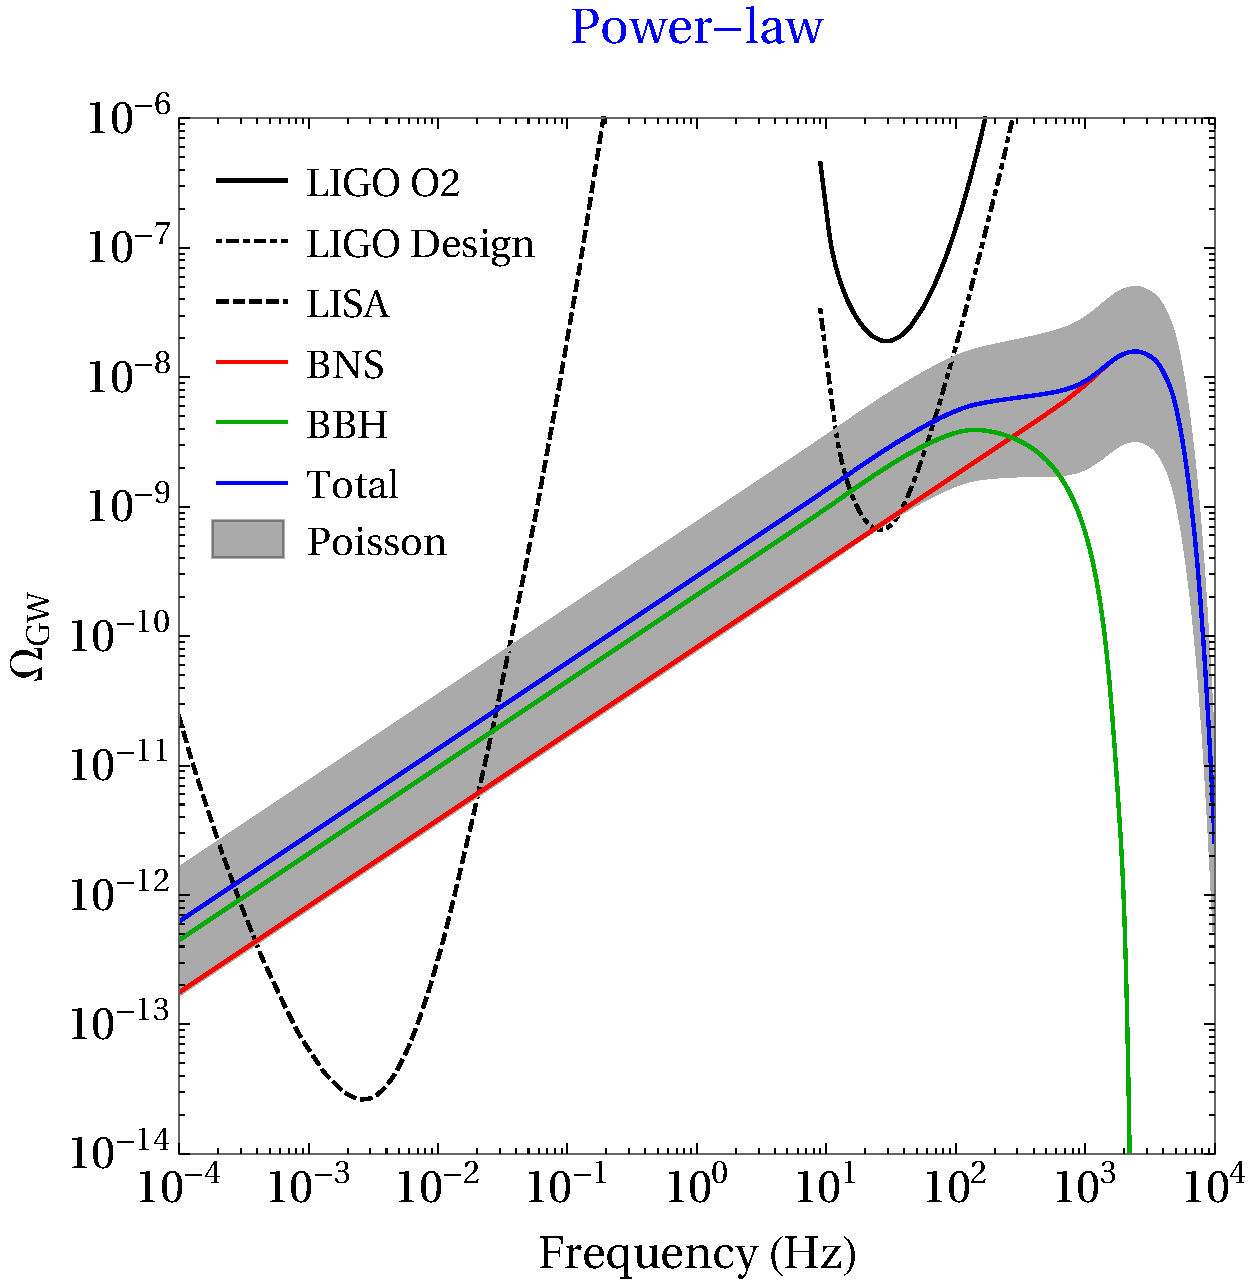
\includegraphics[width = \textwidth]{./pic/omegagw-power.pdf}
            \end{figure}
        \end{column}
        \begin{column}{0.54\textwidth} 
            \begin{figure}[htbp!]
                \centering
                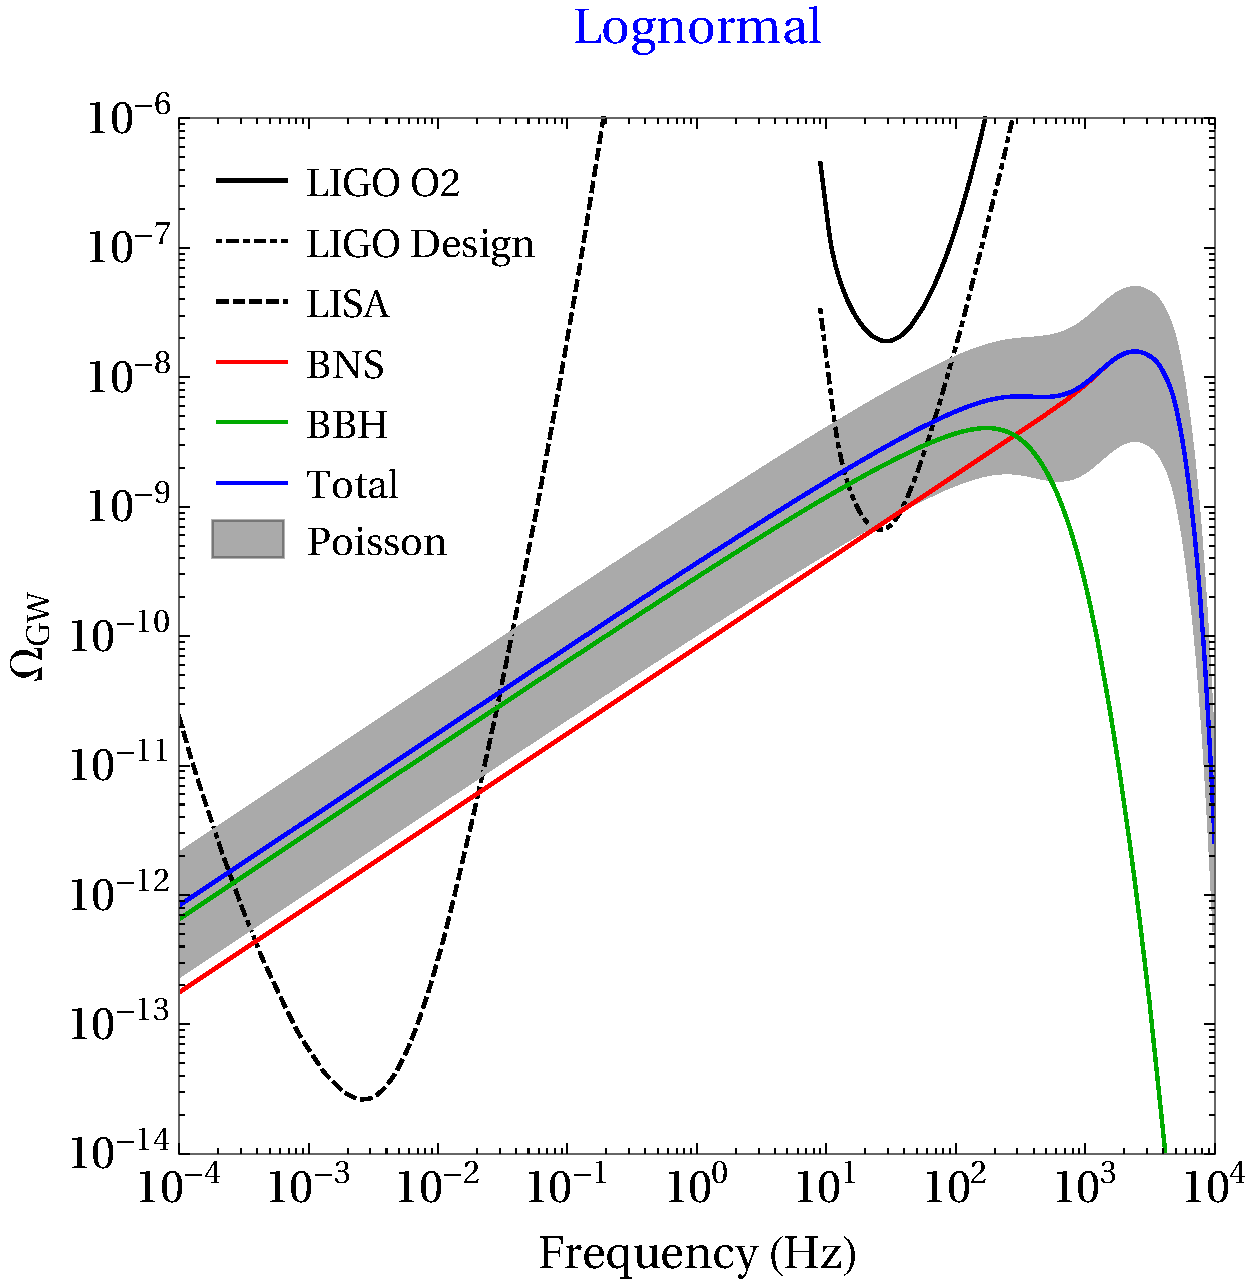
\includegraphics[width = \textwidth]{./pic/omegagw-log.pdf}
            \end{figure}
        \end{column}
    \end{columns}
\end{frame}
%%%%%%%%%%%%%%%%%%%%%%%%%%%%%%%%%%%%%%%%%%%%%%%%%%%%%%%%%%%%%%%%%%%%%%


%%%%%%%%%%%%%%%%%%%%%%%%%%%%%%%%%%%%%%%%%%%%%%%%%%%%%%%%%%%%%%%%%%%%%%
\begin{frame}
    \frametitle{LISA探测随机引力波背景的信噪比(SNR) }\vspace{-3mm}
    \begin{block}{}\vspace{-1mm}\small{
            \[
            \text{SNR}=\sqrt{T} \left[ \int \rmd \nu \frac{\Omega_{\mathrm{GW}}(\nu)}{\Omega_{n}(\nu)} \right]^{1/2}\quad
            \text{其中} \quad
            \Omega_{n}(\nu)\equiv \frac{2 \pi^2 \nu^3 S_{n}(\nu)}{3 H_{0}^2} 
            \]}\vspace{-3mm}
    \end{block}
    \vspace{-4mm}
    \begin{columns}
        \begin{column}{0.52\textwidth} 
            \begin{figure}[htbp!]
                \centering
                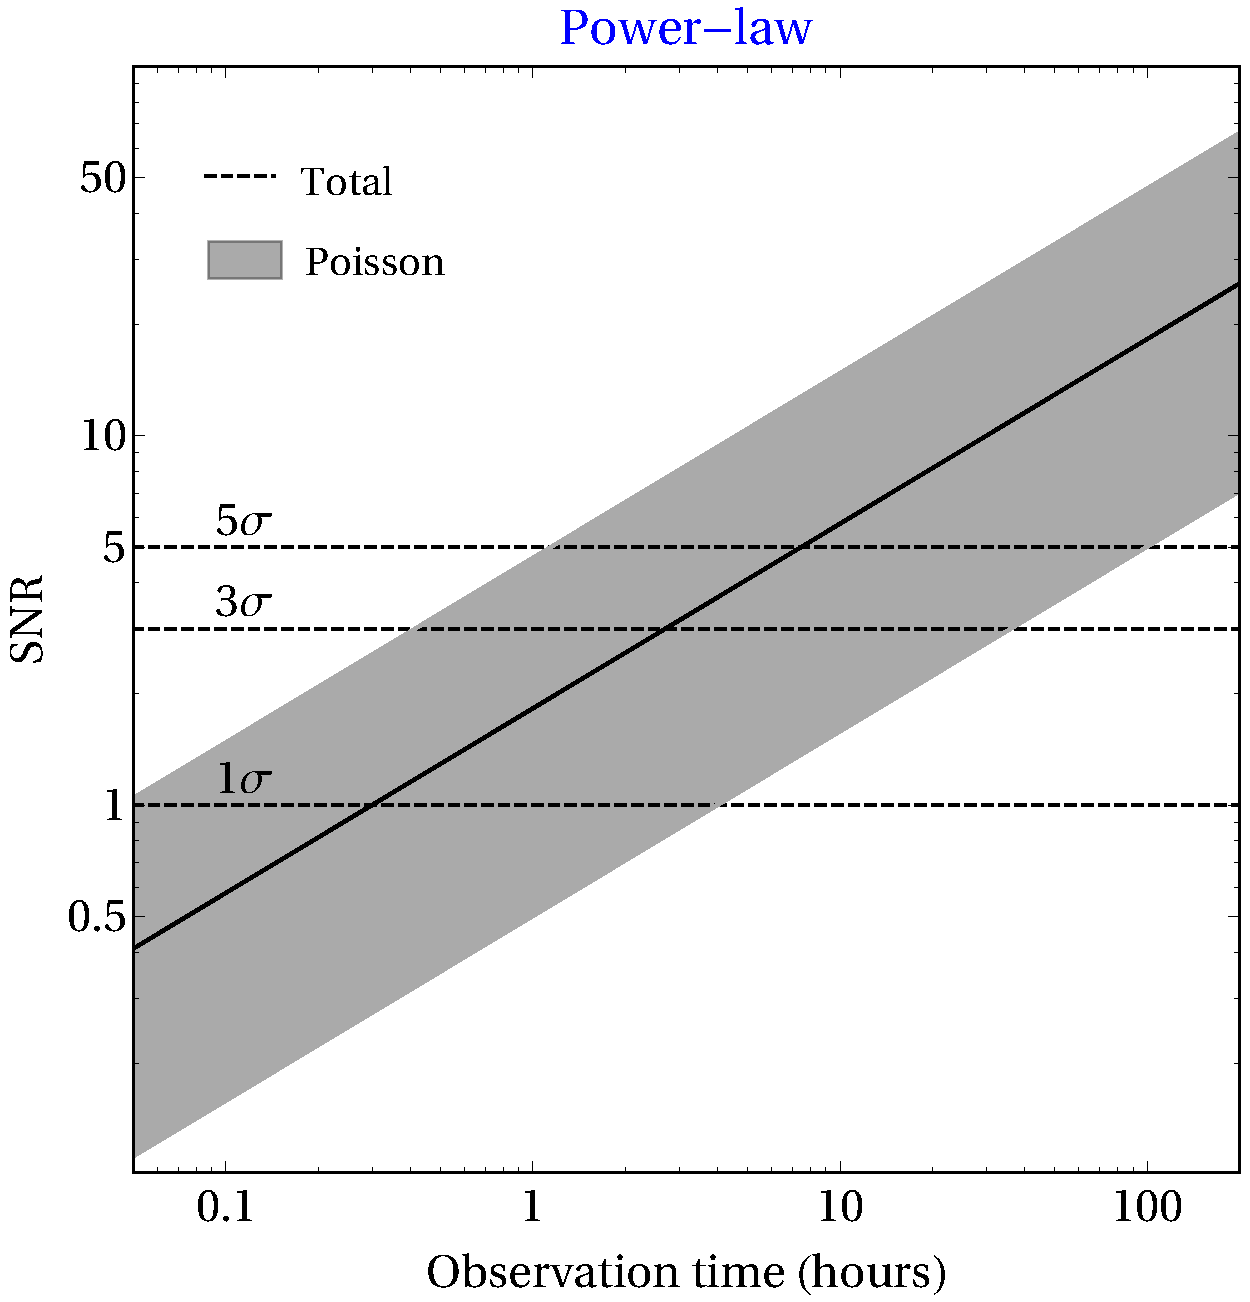
\includegraphics[width = \textwidth]{./pic/snr-power.pdf}
            \end{figure}
        \end{column}
        \begin{column}{0.52\textwidth} 
            \begin{figure}[htbp!]
                \centering
                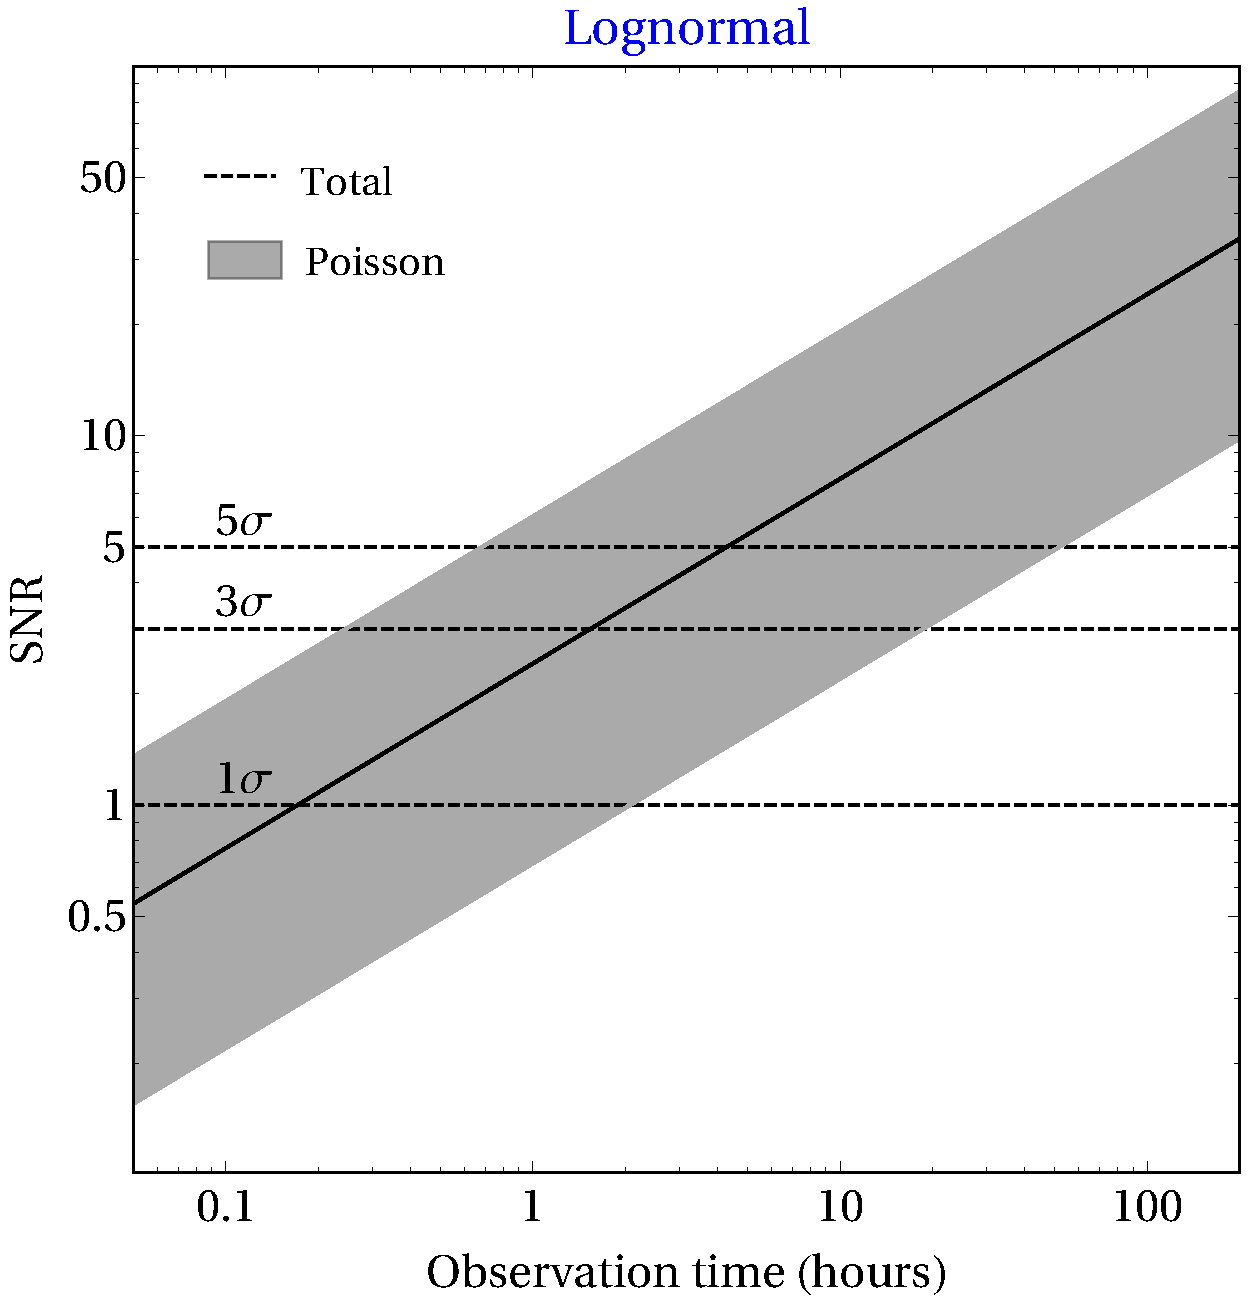
\includegraphics[width = \textwidth]{./pic/snr-log.pdf}
            \end{figure}
        \end{column}
    \end{columns}
\end{frame}
%%%%%%%%%%%%%%%%%%%%%%%%%%%%%%%%%%%%%%%%%%%%%%%%%%%%%%%%%%%%%%%%%%%%%%


%%%%%%%%%%%%%%%%%%%%%%%%%%%%%%%%%%%%%%%%%%%%%%%%%%%%%%%%%%%%%%%%%%%%%%
\begin{frame}
    \frametitle{LISA的额外噪音}
    \vspace{-2mm}
    \begin{block}{}\vspace{-1mm}
        \small{
        \[S_{\mathrm{eff}}(\nu)=S_{n}(\nu)+S_{\mathrm{GW}}(\nu),
        \quad \quad
        S_{\mathrm{GW}}(\nu) \equiv \frac{3 H_{0}^2}{2 \pi^2}
        \frac{\Omega_{\mathrm{GW}}(\nu)}{\nu^3} 
        \]
    }\vspace{-3mm}
    \end{block}
    \vspace{-3mm}
    \begin{columns}
        \begin{column}{0.54\textwidth} 
            \begin{figure}[htbp!]
                \centering
                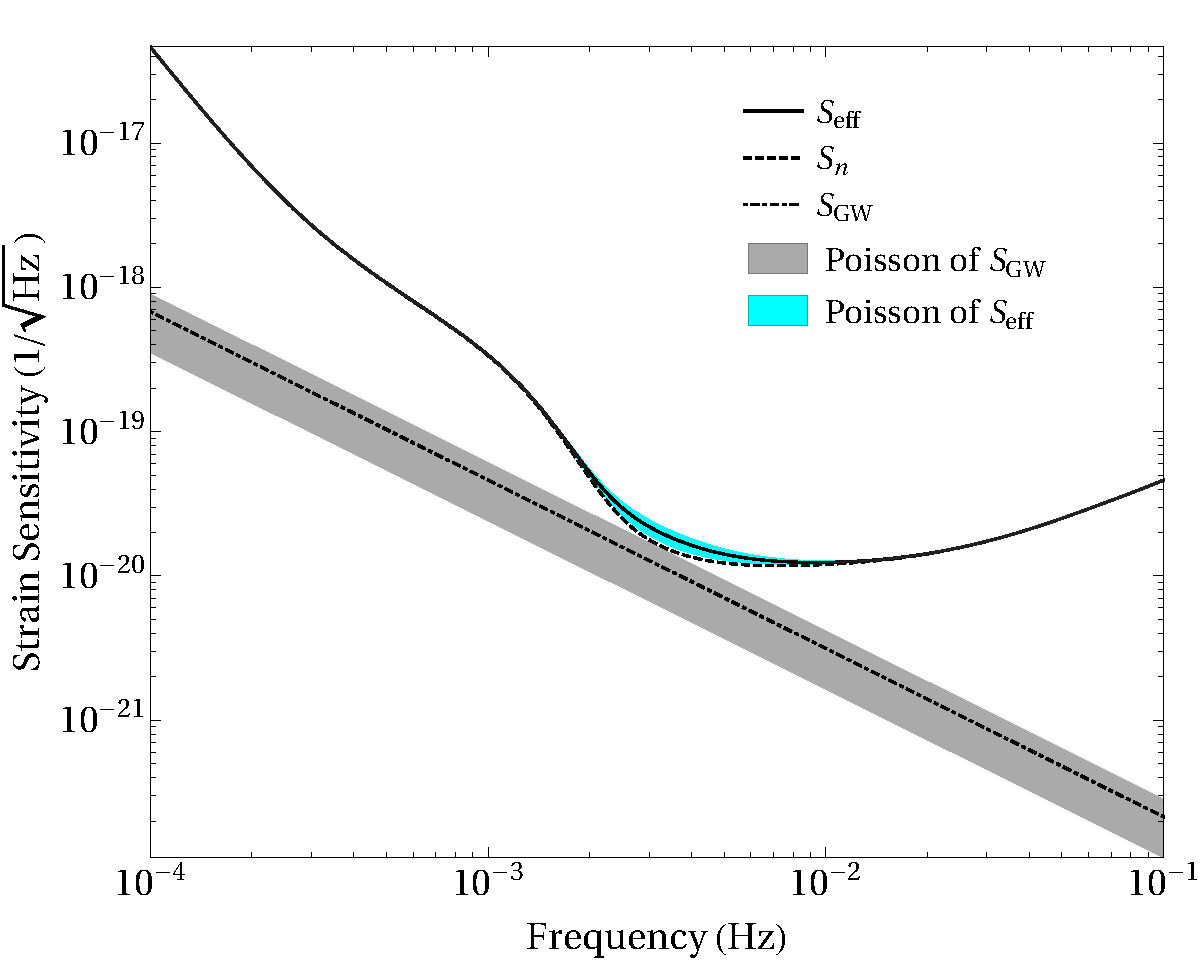
\includegraphics[width = \textwidth]{./pic/lisa-sensitivity-PBH-power.pdf}
            \end{figure}
        \end{column}
        \begin{column}{0.54\textwidth} 
            \begin{figure}[htbp!]
                \centering
                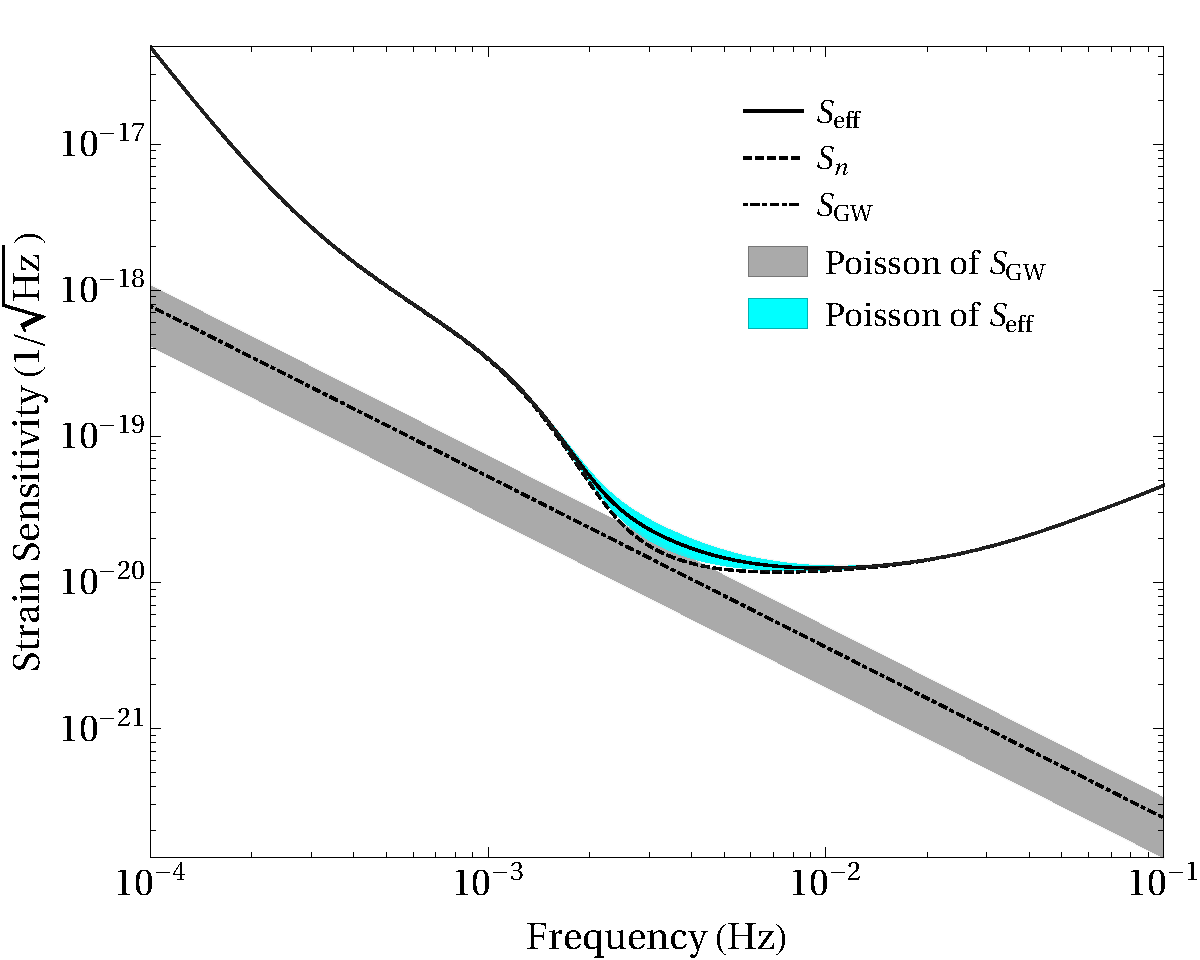
\includegraphics[width = \textwidth]{./pic/lisa-sensitivity-PBH-log.pdf}
            \end{figure}
        \end{column}
    \end{columns}
\end{frame}
%%%%%%%%%%%%%%%%%%%%%%%%%%%%%%%%%%%%%%%%%%%%%%%%%%%%%%%%%%%%%%%%%%%%%%


%%%%%%%%%%%%%%%%%%%%%%%%%%%%%%%%%%%%%%%%%%%%%%%%%%%%%%%%%%%%%%%%%%%%%%
\begin{frame}{降低LISA的探测能力}
    \vspace{-2mm}
    \begin{itemize}
        \item 探测大质量双黑洞的并合是LISA的一个关键科学目标
        \item 降低最大可探测红移 $\Rightarrow$ 降低可探测到的数目
    \end{itemize}
    \vspace{-2mm}
    \begin{columns}
        \begin{column}{0.54\textwidth} 
            \begin{figure}[htbp!]
                \centering
                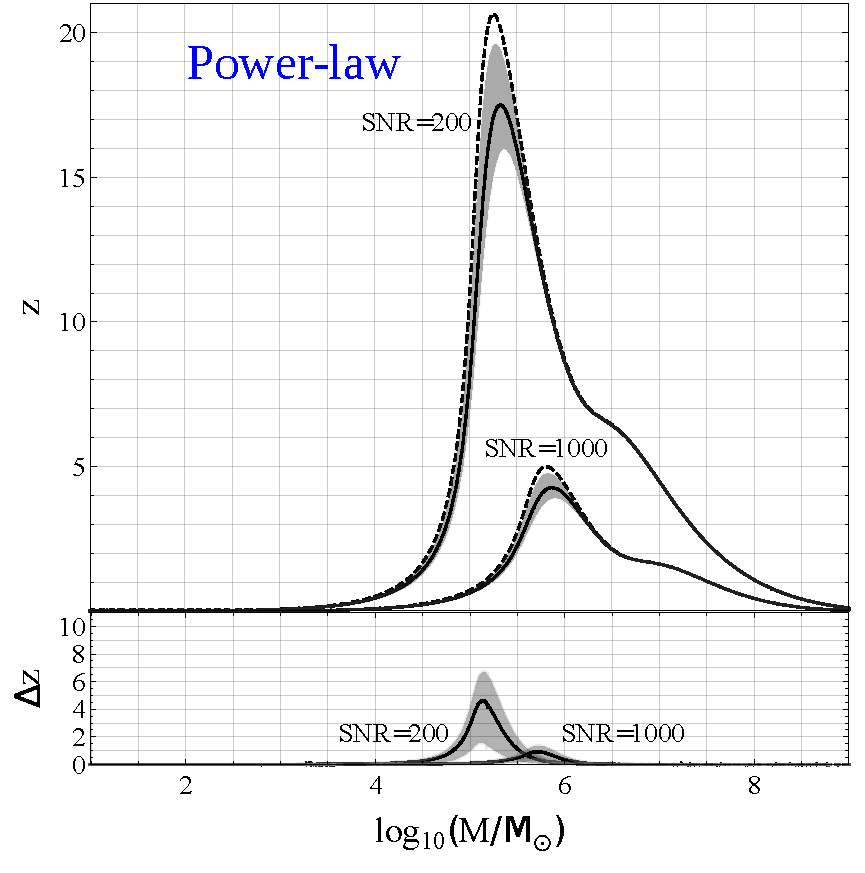
\includegraphics[width = \textwidth]{./pic/z-PBH-power01.pdf}
            \end{figure}
        \end{column}
        \begin{column}{0.54\textwidth} 
            \begin{figure}[htbp!]
                \centering
                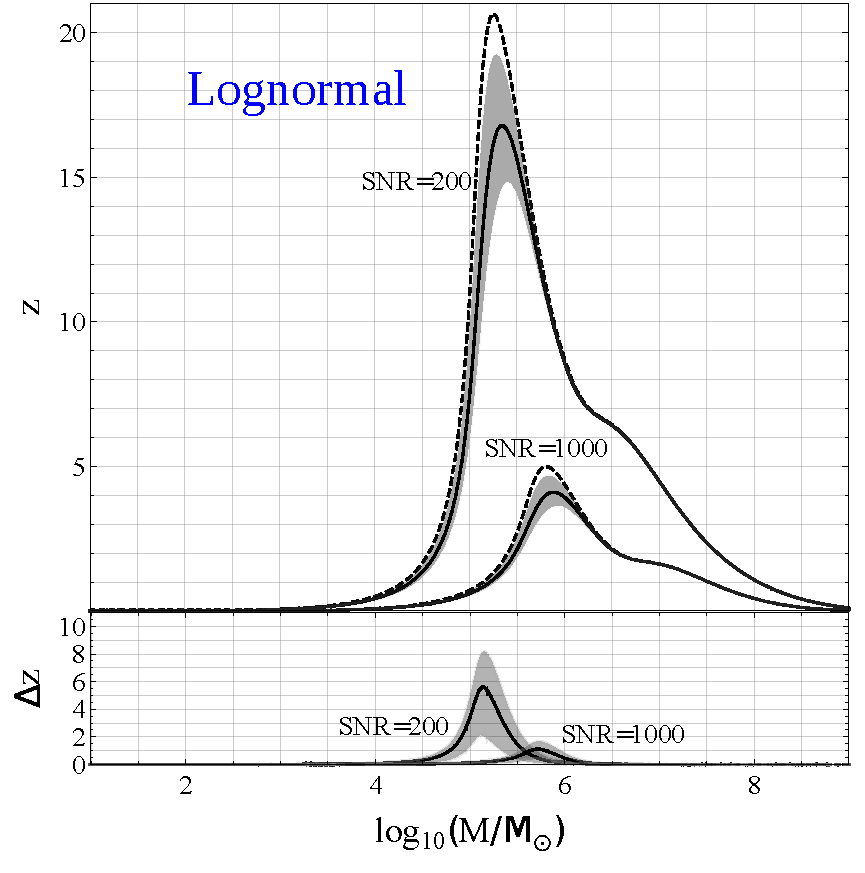
\includegraphics[width = \textwidth]{./pic/z-PBH-log01.pdf}
            \end{figure}
        \end{column}
    \end{columns}
\end{frame}
%%%%%%%%%%%%%%%%%%%%%%%%%%%%%%%%%%%%%%%%%%%%%%%%%%%%%%%%%%%%%%%%%%%%%%

%%%%%%%%%%%%%%%%%%%%%%%%%%%%%%%%%%%%%%%%%%%%%%%%%%%%%%%%%%%%%%%%%%%%%%
\begin{frame}{小结}	
    \begin{itemize}        
        \item 计算了原初双黑洞产生的随机引力波背景。
        \item 此引力波背景可以被LIGO设计阶段和LISA探测到。
        \item 如果此引力波背景没能从LISA的噪音中扣除掉,将会构成LISA的额外噪音,从而降低LISA的探测能力。
    \end{itemize}
\end{frame}
%%%%%%%%%%%%%%%%%%%%%%%%%%%%%%%%%%%%%%%%%%%%%%%%%%%%%%%%%%%%%%%%%%%%%%


%%%%%%%%%%%%%%%%%%%%%%%%%%%%%%%%%%%%%%%%%%%%%%%%%%%%%%%%%%%%%%%%%%%%%%

\section{区分原初黑洞和天体物理黑洞}
\subsection{}
%%%%%%%%%%%%%%%%%%%%%%%%%%%%%%%%%%%%%%%%%%%%%%%%%%%%%%%%%%%%%%%%%%%%%%
\begin{frame}{研究动机}
    
    \begin{itemize}
        \item 原初黑洞可以解释\lvc 探测到的双黑洞并合事件。
        \item \red{如何判断探测到的黑洞是原初黑洞还是天体物理黑洞?}
        \begin{itemize}
            \item 亚太阳质量的黑洞必然是原初黑洞
            \item 黑洞的群体性质(例如红移分布)$\Rightarrow$判断超太阳质量的黑洞的起源
        \end{itemize}
    \end{itemize}
\end{frame}
%%%%%%%%%%%%%%%%%%%%%%%%%%%%%%%%%%%%%%%%%%%%%%%%%%%%%%%%%%%%%%%%%%%%%%
%%%%%%%%%%%%%%%%%%%%%%%%%%%%%%%%%%%%%%%%%%%%%%%%%%%%%%%%%%%%%%%%%%%%%%
\begin{frame}{第三代地基引力波探测器}
    \begin{columns}
        \begin{column}{0.6\textwidth} 
            \begin{figure}[htbp!]
                \centering
                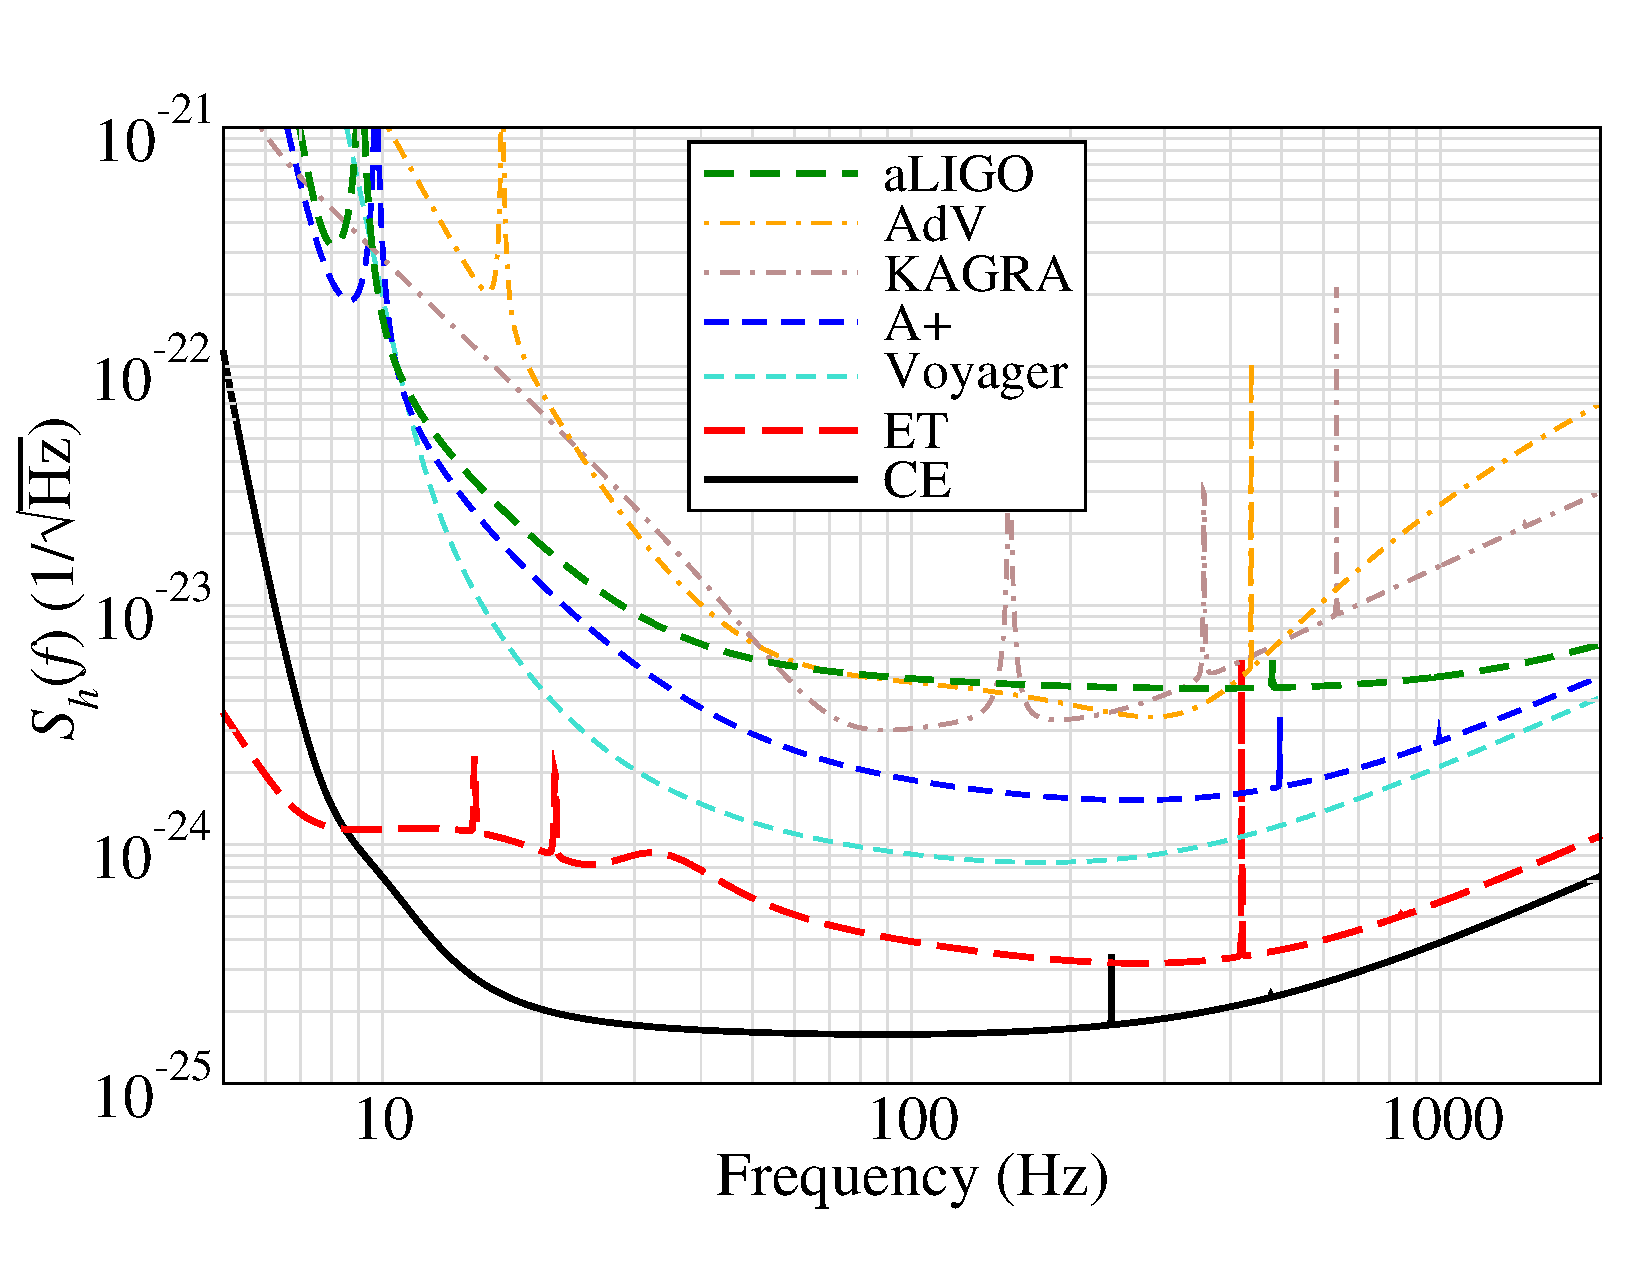
\includegraphics[width=\textwidth]{et_ce_sn}
            \end{figure}
        \end{column}
        \begin{column}{0.52\textwidth} 
            \begin{figure}[htbp!]
                \centering
                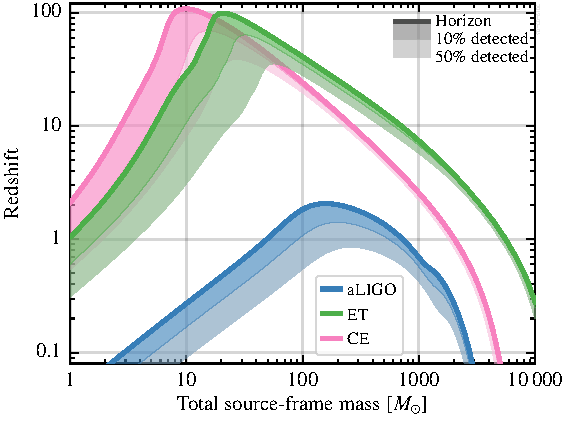
\includegraphics[width=\textwidth]{gw_horizons}
            \end{figure}
        \end{column}
    \end{columns}
    \vspace{-1mm}
    \begin{itemize}
        \item ET和CE可以探测更低的频率和更高的红移
        \item ET和CE有望每年探测到$\Od(10^5)$个双黑洞并合事件 \Refs{Phys. Rev. Lett. 118, 151105 (2017)}
    \end{itemize}
\end{frame}
%%%%%%%%%%%%%%%%%%%%%%%%%%%%%%%%%%%%%%%%%%%%%%%%%%%%%%%%%%%%%%%%%%%%%%


%%%%%%%%%%%%%%%%%%%%%%%%%%%%%%%%%%%%%%%%%%%%%%%%%%%%%%%%%%%%%%%%%%%%%%
\begin{frame}{亚太阳质量的情况——单色质量谱}
    \centering
    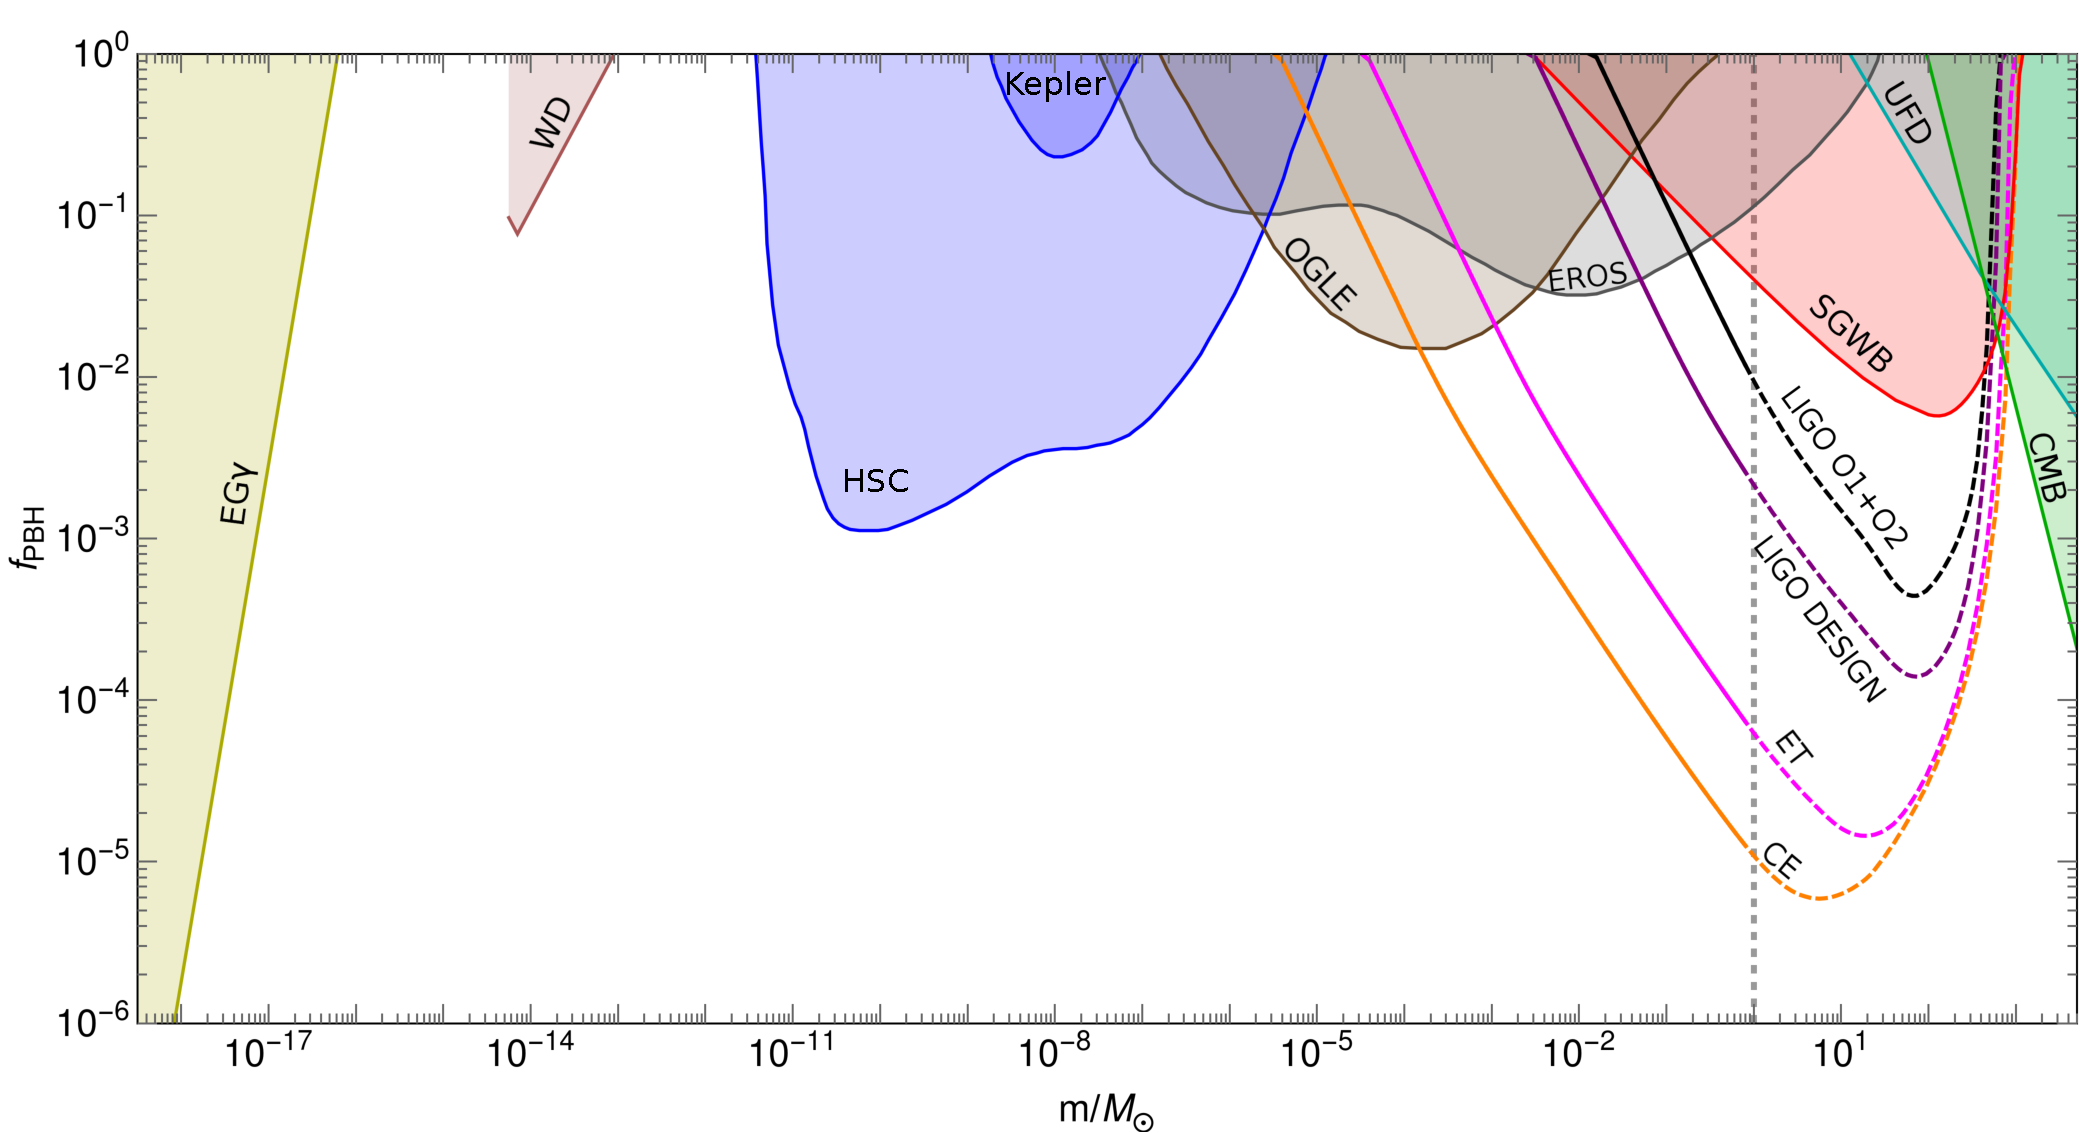
\includegraphics[width=\textwidth]{fpbh_m.pdf}
\end{frame}


%%%%%%%%%%%%%%%%%%%%%%%%%%%%%%%%%%%%%%%%%%%%%%%%%%%%%%%%%%%%%%%%%%%%%%
\begin{frame}{亚太阳质量的情况——一般质量谱}
    \begin{itemize}
        \item 用分段的方法重构质量函数
        
        \e\label{para} 
        P(m) = \begin{cases} 
            P_0, & 0.2\, \Msun \leq m < 1\, \Msun \\
            P_1, & 1\, \Msun \leq m < 30\, \Msun \\
            P_2, & 30\, \Msun \leq m < 60\, \Msun \\
            P_3, & 60\, \Msun \leq m \leq 100\, \Msun
        \end{cases}
        \q 
        
        \item 其中$P_i = \{ P_0, P_1, P_2, P_3 \} $为四个常数,其满足归一化条件
        \e 
        \int P(m)\, \rd m = 0.8P_0 + 29P_1 + 30P_2 + 40P_3 = 1.
        \q 
        
        \item 四个$P_i$中只有三个是独立的,我们选择$\vth = \{P_1, P_2, P_3\}$作为自由参数。
        
        \item 用GWTC-1(O1和O2)的10个双黑洞并合事件去拟合$\vth$。
    \end{itemize}    
\end{frame}


%%%%%%%%%%%%%%%%%%%%%%%%%%%%%%%%%%%%%%%%%%%%%%%%%%%%%%%%%%%%%%%%%%%%%%
\begin{frame}{搜索具有亚太阳质量和超太阳质量的双黑洞}
    \vspace{-2mm}
    \begin{block}{}\vspace{-1mm}\small{
            \[
            \{R,\, \fpbh\} = \{308^{+193}_{-135}\, \gpcyr,\ 3.3\,^{+2.3}_{-1.8} \times 10^{-3}\}
            \]
        }
    \vspace{-4mm}
    \end{block}  
    \vspace{-1mm}
    \begin{figure}[h!]
        \centering
        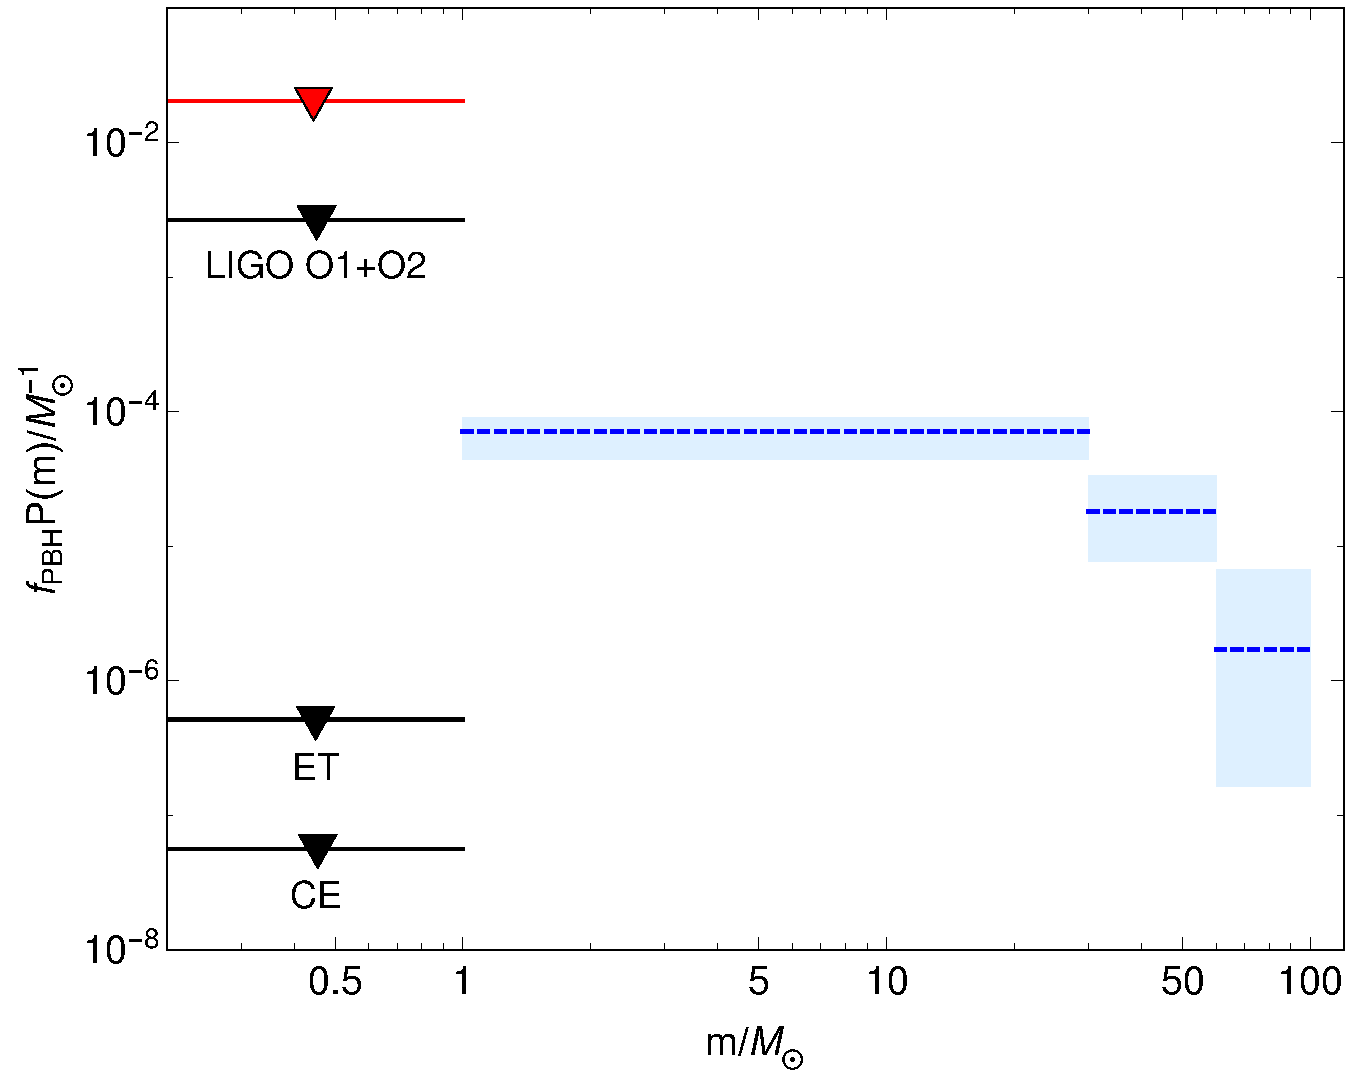
\includegraphics[width=0.75\textwidth]{fpbhPmdm.pdf}
    \end{figure}
\end{frame}

%%%%%%%%%%%%%%%%%%%%%%%%%%%%%%%%%%%%%%%%%%%%%%%%%%%%%%%%%%%%%%%%%%%%%%
\begin{frame}{超太阳质量的情况:原初双黑洞并合率}
    
    \begin{tcolorbox}[ams align,colback=white!10!yellow]
        \mR_{12}(t) \approx&\, 3.9\cdot 10^6\times \red{\({t\over t_0}\)^{-{34\over 37}}} f^2 (f^2+\sigma_{\rm{eq}}^2)^{-{21\over 74}} \nonumber \\
        & \times  \min\(\frac{P(m_1)}{m_1}, \frac{P(m_2)}{m_2}\) \({P(m_1)\over m_1}+{P(m_2)\over m_2}\) \nonumber \\
        & \times (m_1 m_2)^{{3\over 37}} (m_1+m_2)^{36\over 37}\nonumber
    \end{tcolorbox}
    
    \begin{itemize}       
        \vspace{-2mm}
        \item 原初黑洞占冷暗物质的丰度$f_{\rm{PBH}}\equiv \Omega_{\rm{PBH}}/\Omega_{\rm{CDM}} \approx f/0.85$
        \item $\sigma_{\rm{eq}} \sim 0.005$是其它暗物质密度扰动的方差。
        \item 红移越大的时候,并合率越大$\Rightarrow$区分原初黑洞和天体物理黑洞
        
    \end{itemize}
\end{frame}
%%%%%%%%%%%%%%%%%%%%%%%%%%%%%%%%%%%%%%%%%%%%%%%%%%%%%%%%%%%%%%%%%%%%%%

%%%%%%%%%%%%%%%%%%%%%%%%%%%%%%%%%%%%%%%%%%%%%%%%%%%%%%%%%%%%%%%%%%%%%%
\begin{frame}{超太阳质量的情况:天体物理双黑洞并合率}
    并合率是天体物理黑洞的生成率$R_{\mathrm{birth}}(z,m)$与天体物理双黑洞的时间延迟分布$P_d(t_d)$的卷积\Refs{Mon.Not.Roy.Astron.Soc. 461 (2016) 4, 3877-3885}
    \e\label{sBHR}
    \mR_{12}(z) = \int^{t_{\mathrm{max}}}_{t_{\text{min}}}  
    \frac{R_{\mathrm{birth}}(t(z)-t_d, m_1)}{m_1-5\Msun} \times P_d (t_d)\ d t_d,
    \q
    其中$t_d$是时间延迟,$t(z)$双黑洞并合时的宇宙年龄。
    \begin{itemize}
        \item \texttt{Fiducial}模型:$R_{\mathrm{birth}}$由发光星系观测结果拟合得到,$P_{d} \propto t_{d}^{-1}$,$t_{\mathrm{min}} = 50$\,Myr,$t_{\mathrm{max}}$为哈勃时间。
        
        \item \texttt{GRB-based}模型:$R_{\mathrm{birth}}$由高红移下的伽马射线暴(GRB)校准而得到。
        
        \item \texttt{LongDelay}模型:与\texttt{Fiducial}模型基本相同,但$t_{\mathrm{min}}=5$Gyr。
        
        \item \texttt{FlatDelay} 模型:$P_{d}$是平的分布,$t_{\mathrm{min}}=50$Myr,且$t_{\mathrm{max}}=1$Gyr。
    \end{itemize}    
\end{frame}

%%%%%%%%%%%%%%%%%%%%%%%%%%%%%%%%%%%%%%%%%%%%%%%%%%%%%%%%%%%%%%%%%%%%%%
\begin{frame}{}
    \begin{figure}[h!]
        \centering
        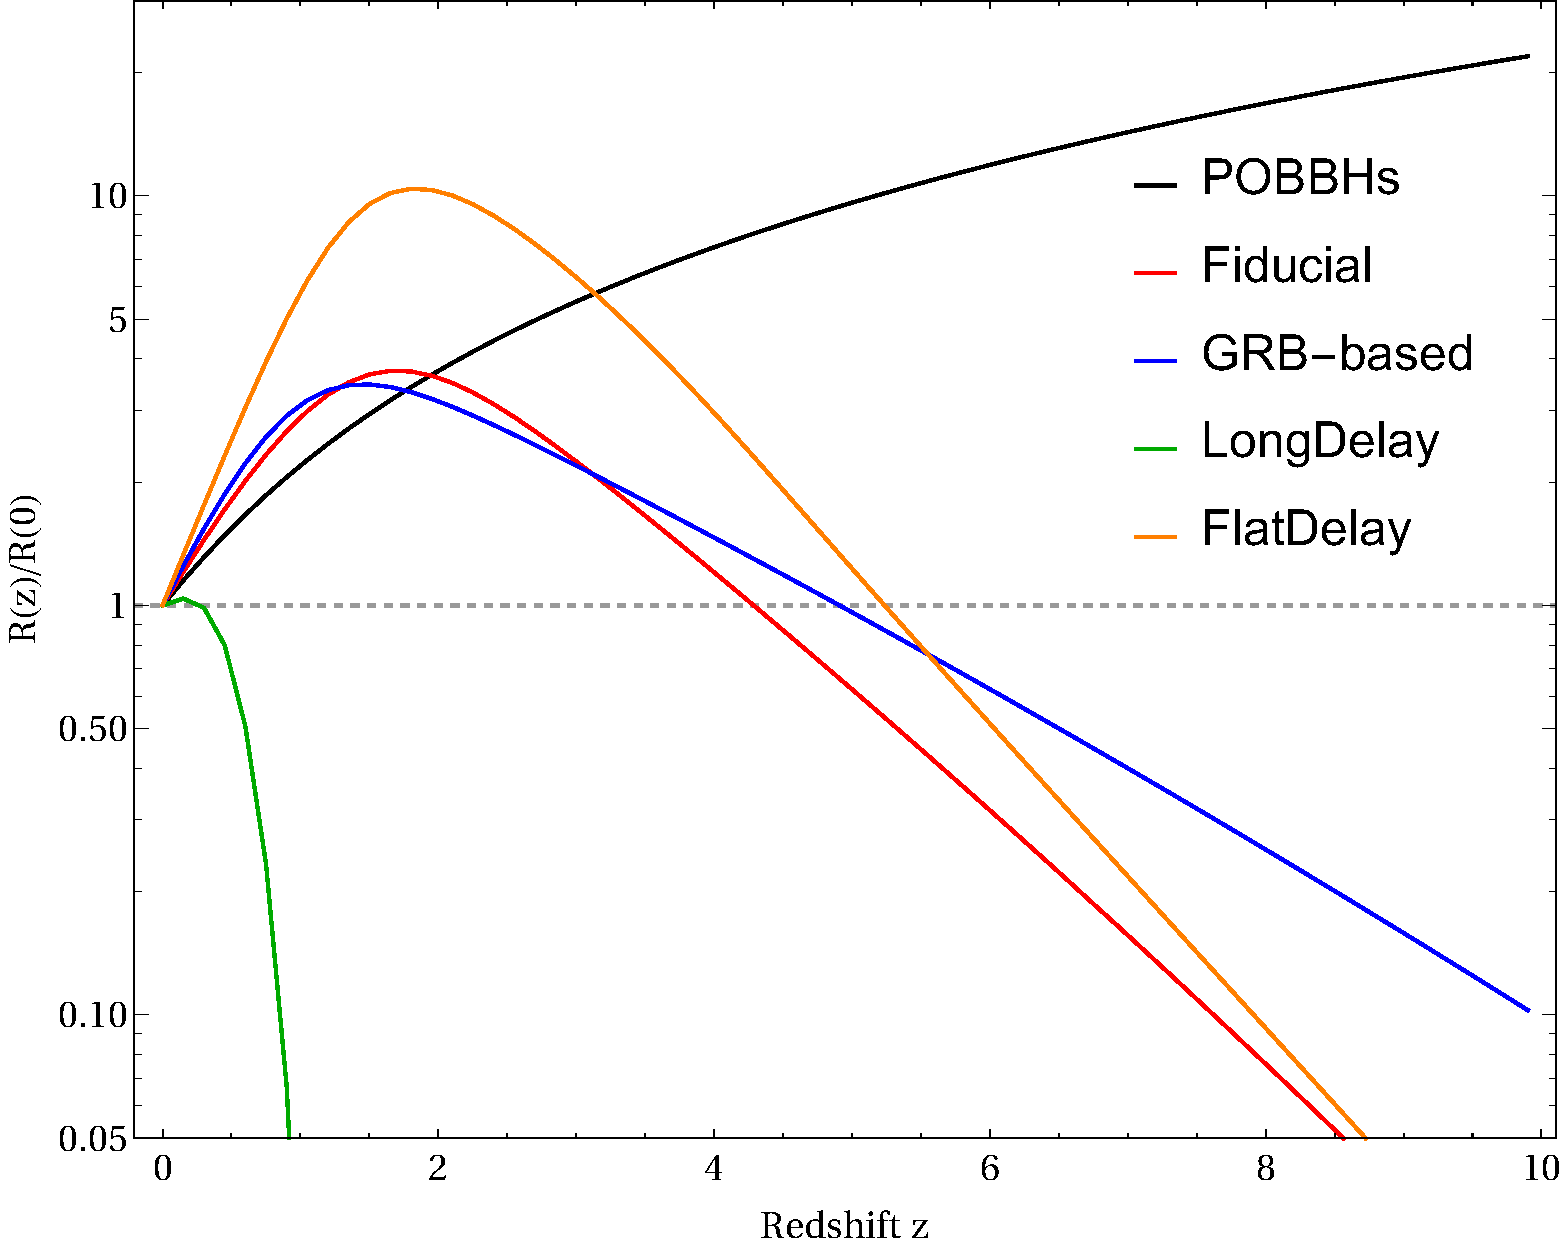
\includegraphics[width=0.8\textwidth]{R_z.pdf}
        \caption{
            原初双黑洞(POBBHs)和天体物理双黑洞给出的归一化并合率$R(z)/R(0)$的红移分布。双黑洞的质量范围为$5\Msun \sim 100 \Msun$。 
        }
    \end{figure}
\end{frame}

%%%%%%%%%%%%%%%%%%%%%%%%%%%%%%%%%%%%%%%%%%%%%%%%%%%%%%%%%%%%%%%%%%%%%%
\begin{frame}{通过红移演化来区分原初黑洞和天体物理黑洞}
    \vspace{-3mm}
    \begin{block}{}\small{
            \[ \text{可观测事件数} \quad
            \Nobs (z) = \int \rd m_1 \rd m_2\, \int_0^z \mR_{12}(z')\,
            \frac{\rd VT}{\rd z'} \rd z'
            \]}\vspace{-3mm}
    \end{block}
    \vspace{-1mm}
    \begin{columns}
        \begin{column}{0.55\textwidth} 
            \begin{figure}[htbp!]
                \centering
                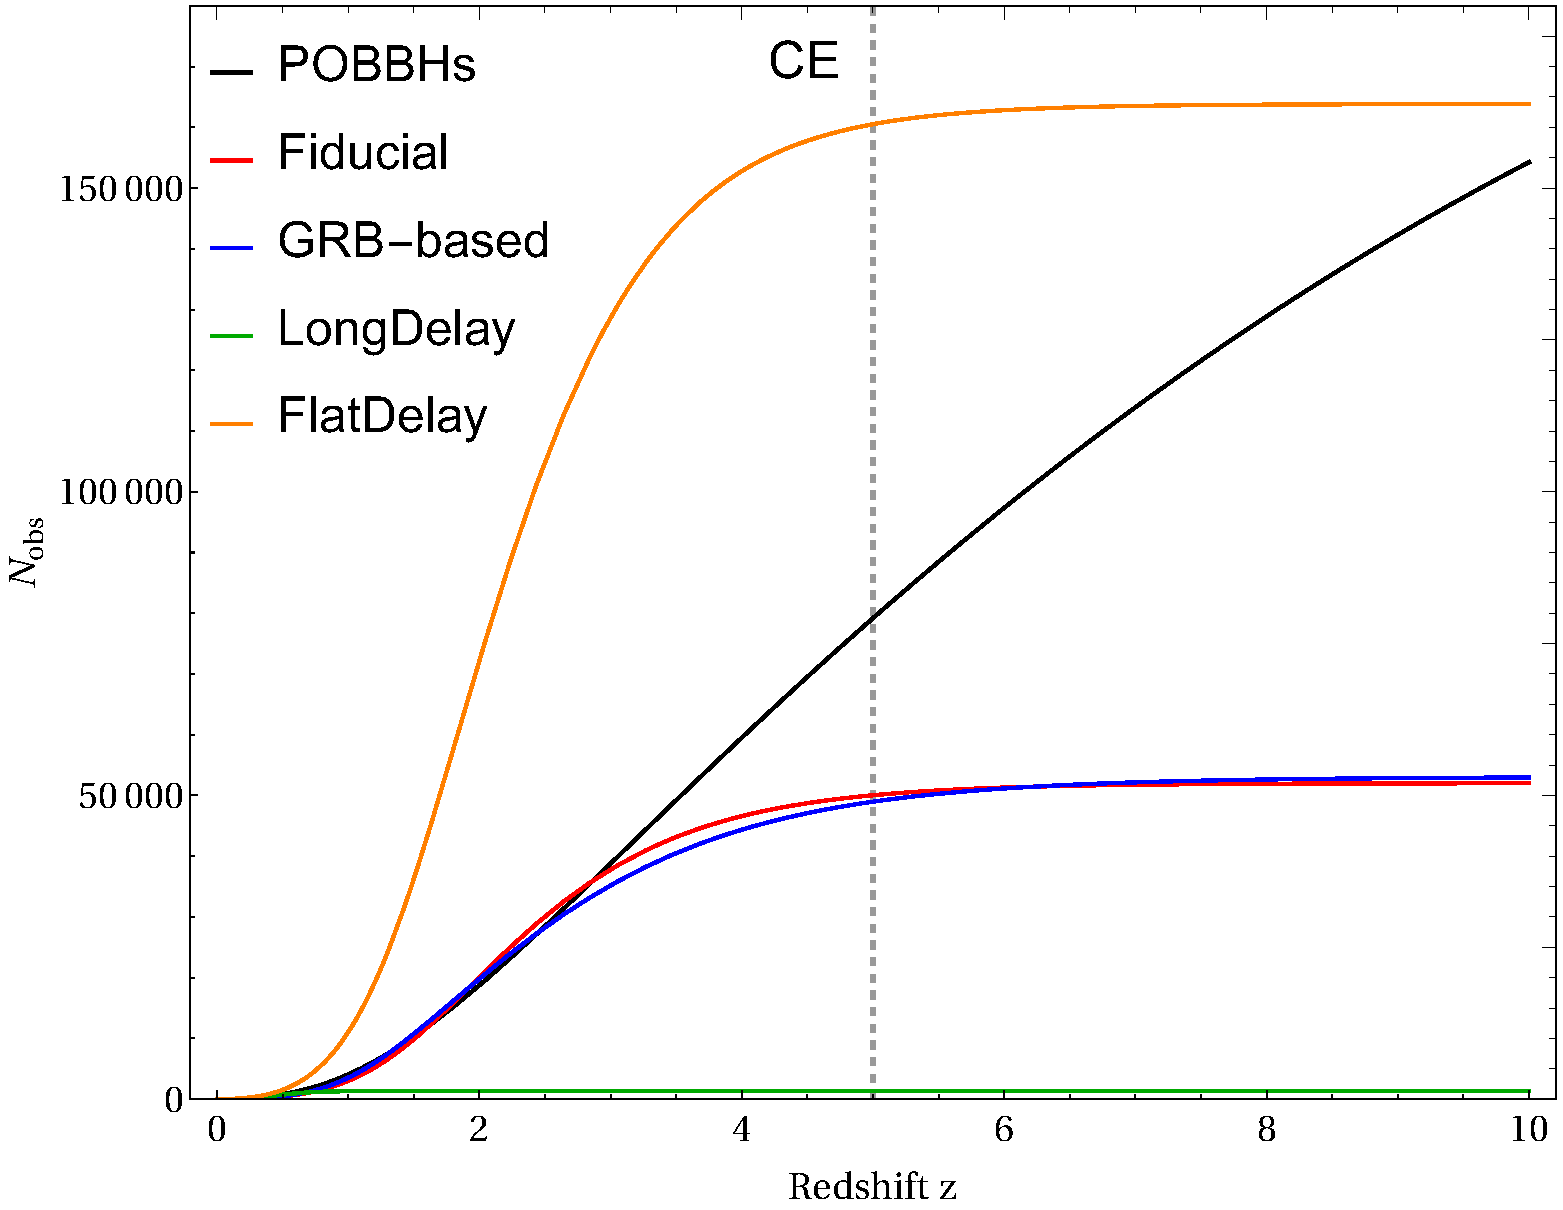
\includegraphics[width = \textwidth]{events_CE.pdf}
            \end{figure}
        \end{column}
        \begin{column}{0.55\textwidth} 
            \begin{figure}[htbp!]
                \centering
                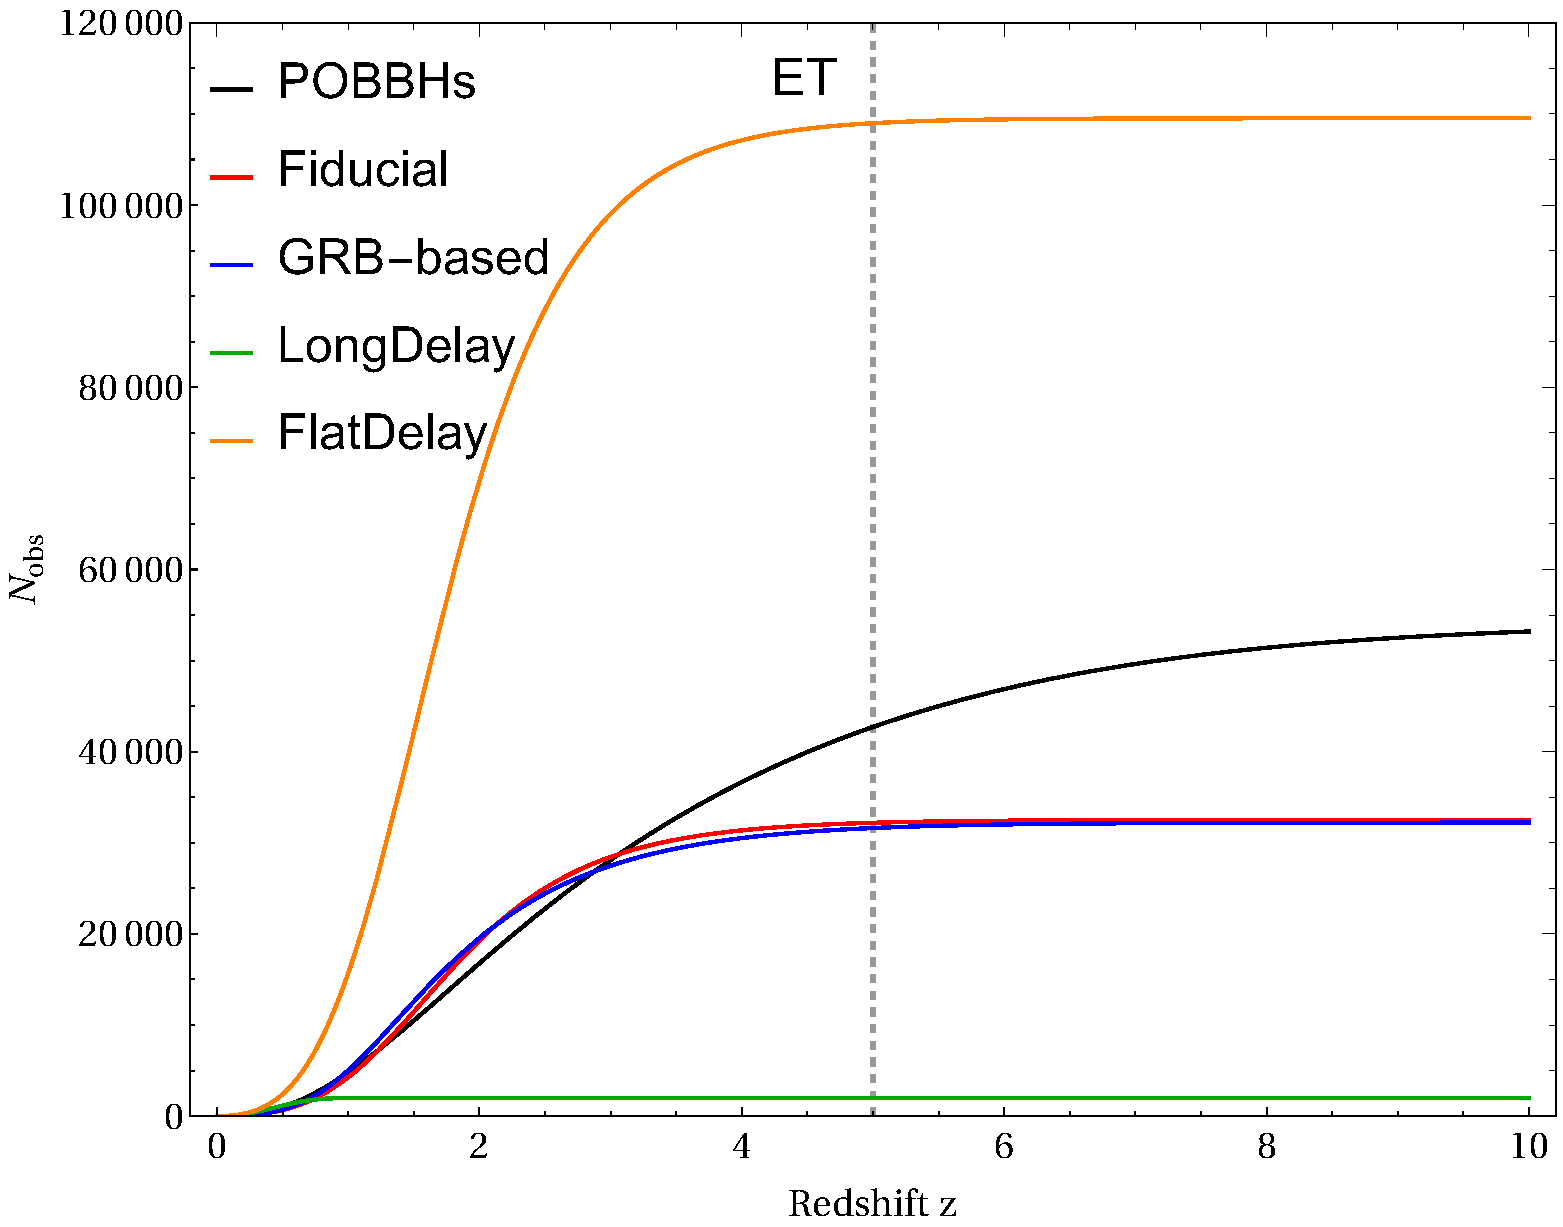
\includegraphics[width = \textwidth]{events_ET.pdf}
            \end{figure}
        \end{column}
    \end{columns}
\centering
\red{看红移$z>5$时的$\Nobs$的变化}
\end{frame}
%%%%%%%%%%%%%%%%%%%%%%%%%%%%%%%%%%%%%%%%%%%%%%%%%%%%%%%%%%%%%%%%%%%%%%
%%%%%%%%%%%%%%%%%%%%%%%%%%%%%%%%%%%%%%%%%%%%%%%%%%%%%%%%%%%%%%%%%%%%%%
\begin{frame}{小结}	
    \begin{itemize}        
        \item 探讨如何通过第三代地基引力波探测器来区分原初黑洞和天体物理黑洞。
        \item 通过定向搜寻至少包含一个亚太阳质量的双黑洞系统,估算了$\fpbh$的可探测极限。
        \item 预测了ET和CE能够探测到的双黑洞事件数目随红移的分布,从而来区分原初黑洞和天体物理黑洞。
    \end{itemize}
\end{frame}
%%%%%%%%%%%%%%%%%%%%%%%%%%%%%%%%%%%%%%%%%%%%%%%%%%%%%%%%%%%%%%%%%%%%%%
%%%%%%%%%%%%%%%%%%%%%%%%%%%%%%%%%%%%%%%%%%%%%%%%%%%%%%%%%%%%%%%%%%%%%%

\section[PTA限制$\fpbh$]{用脉冲星计时阵列限制原初黑洞丰度的限制}
%\subsection{}

%%%%%%%%%%%%%%%%%%%%%%%%%%%%%%%%%%%%%%%%%%%%%%%%%%%%%%%%%%%%%%%%%%%%%%
\begin{frame}{研究动机}
    \begin{itemize}
        \item 除了直接探测原初双黑洞及其产生的随机引力波背景外,还有间接的方法来探测原初黑洞。
        \item 在原初黑洞形成的过程中,标量扰动将不可避免地产生诱导引力波
        {\small
        \e
        \rd s^{2}=a^{2}\left\{-(1+2 \phi) \rd \eta^{2}+\left[(1-2 \phi) \delta_{i j}+\frac{h_{i j}}{2}\right] \rd x^{i} \rd x^{j}\right\},
        \q
    }
        其中$\phi \equiv \phi^{(1)}$是标量扰动,$h_{ij} \equiv h_{ij}^{(2)}$为张量扰动。
        
        \item 考虑单色质量谱,则相应曲率扰动$\zeta= (3/2)\phi$的功率谱为
        \e\label{pzeta1}
        \mathcal{P}_{\zeta}(k)=A k_*\delta\(k-k_*\).
        \q
        
        \item \red{通过探测标量诱导引力波可以间接探测原初黑洞}
        {\small
        \e\label{fpbh}
        f_{\mathrm{PBH}} \simeq 1.9 \times 10^{7}
        \(\frac{1}{A}-1\) e^{-{1\over 2A}} \left(\frac{m_{\mathrm{PBH}}}{M_{\odot}}\right)^{-\frac{1}{2}}.
        \q
    }
    \end{itemize}
\end{frame}
%%%%%%%%%%%%%%%%%%%%%%%%%%%%%%%%%%%%%%%%%%%%%%%%%%%%%%%%%%%%%%%%%%%%%%


%%%%%%%%%%%%%%%%%%%%%%%%%%%%%%%%%%%%%%%%%%%%%%%%%%%%%%%%%%%%%%%%%%%%%%
\begin{frame}{三阶标量诱导引力波}
    \vspace{-3mm}
        \small{\[
            h_{i j}^{\prime \prime}+2 \mathcal{H} h_{i j}^{\prime}-\nabla^{2} h_{i j}=-4 \mathcal{T}_{i j}^{\ell m} S_{\ell m}
            \]
            \[
            \ogw(\eta, k)=\frac{1}{\rho_c} \frac{d\rho_{\mathrm{GW}}}{d \ln f} \propto \avg{S^{(2)}S^{(2)}} + \avg{S^{(3)}S^{(3)}} + \avg{S^{(2)}S^{(4)}}
            \]}
           {\tiny \[
            \Sij{2}= 4 \phi \p_i\p_j\phi + 2\p_i\phi\p_j\phi-\p_i \(\phi + {\phi'\over\mH}\)
            \p_j\(\phi + {\phi'\over\mH}\)
            \]            
            \[
            \begin{split}
                \Sij{3} =& \frac{1}{\mH} \(12\mH \phi - \phi'\) \p_i\phi \p_j\phi
                - \frac{1}{\mH^3} \(4\mH \phi - \phi'\)\p_i\phi'\p_j\phi' \\
                &+ \frac{1}{3\mH^4} \(2\p^2\phi - 9\mH \phi'\) \p_i\(\mH\phi +\phi'\)
                \p_j\(\mH\phi +\phi'\)
            \end{split}
            \]            
            \[
            \begin{split}
                \Sij{4} =& 16 \phi^3 \p_i\p_j\phi
                + \frac{1}{3\mH^3} \Big[2 \phi' \p^2\phi - 9\mH \phi'^2 
                - 8\mH \phi \p^2\phi + 18 \mH^2 \phi \phi'
                + 96\mH^3 \phi^2\Big] \p_i\phi\p_j\phi \\
                &+ \frac{2}{3\mH^5} \Big[- \phi' \p^2\phi + 3\mH \phi'^2 
                + 4\mH \phi \p^2\phi + 3 \mH^2 \phi \phi'- 12\mH^3 \phi^2\Big] \p_i\phi' \p_j\phi'\\
                &+ \frac{1}{36\mH^6} \Big[ 
                -16 (\p^2\phi)^2 - 3  \partial_k\phi' \partial^k\phi'
                + 120 \mH \phi' \p^2\phi - 6 \mH \partial_k\phi \partial^k\phi'	\\
                &\qquad\qquad + 144 \mH^2 \phi \p^2\phi - 180 \mH^2 \phi'^2 
                + 33 \mH^2 \partial_k\phi \partial^k\phi- 504 \mH^3 \phi \phi'
                - 144 \mH^4 \phi^2
                \Big] \\
                &\qquad\qquad\times  \p_i\(\mH\phi +\phi'\)
                \p_j\(\mH\phi +\phi'\)
            \end{split}
            \]
        }
\end{frame}

%%%%%%%%%%%%%%%%%%%%%%%%%%%%%%%%%%%%%%%%%%%%%%%%%%%%%%%%%%%%%%%%%%%%%%
\begin{frame}{标量诱导引力波的能量密度谱}
        \centering
        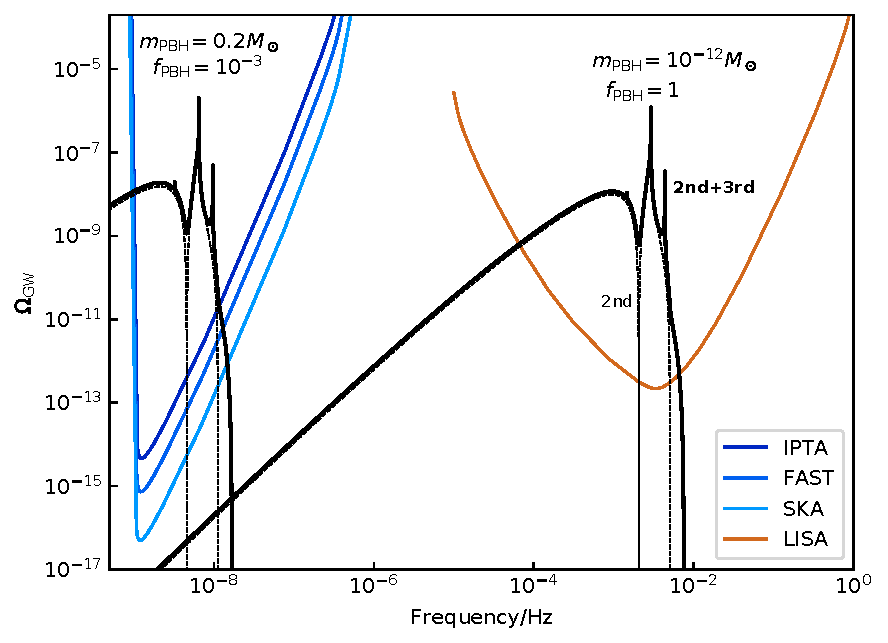
\includegraphics[width=0.8\textwidth]{pic/OmegaGW.pdf}
        \begin{itemize}
            \item 三阶贡献$\sim10\%$的修正;\qquad 把截断频率从$2k_*$延展到$3k_*$
        \end{itemize}
    \centering
    \red{现有的PTA中是否有标量诱导引力波的信号?}
\end{frame}
%%%%%%%%%%%%%%%%%%%%%%%%%%%%%%%%%%%%%%%%%%%%%%%%%%%%%%%%%%%%%%%%%%%%%%

%%%%%%%%%%%%%%%%%%%%%%%%%%%%%%%%%%%%%%%%%%%%%%%%%%%%%%%%%%%%%%%%%%%%%%
\begin{frame}{脉冲星计时阵列(PTA)探测引力波背景}
    \centering
    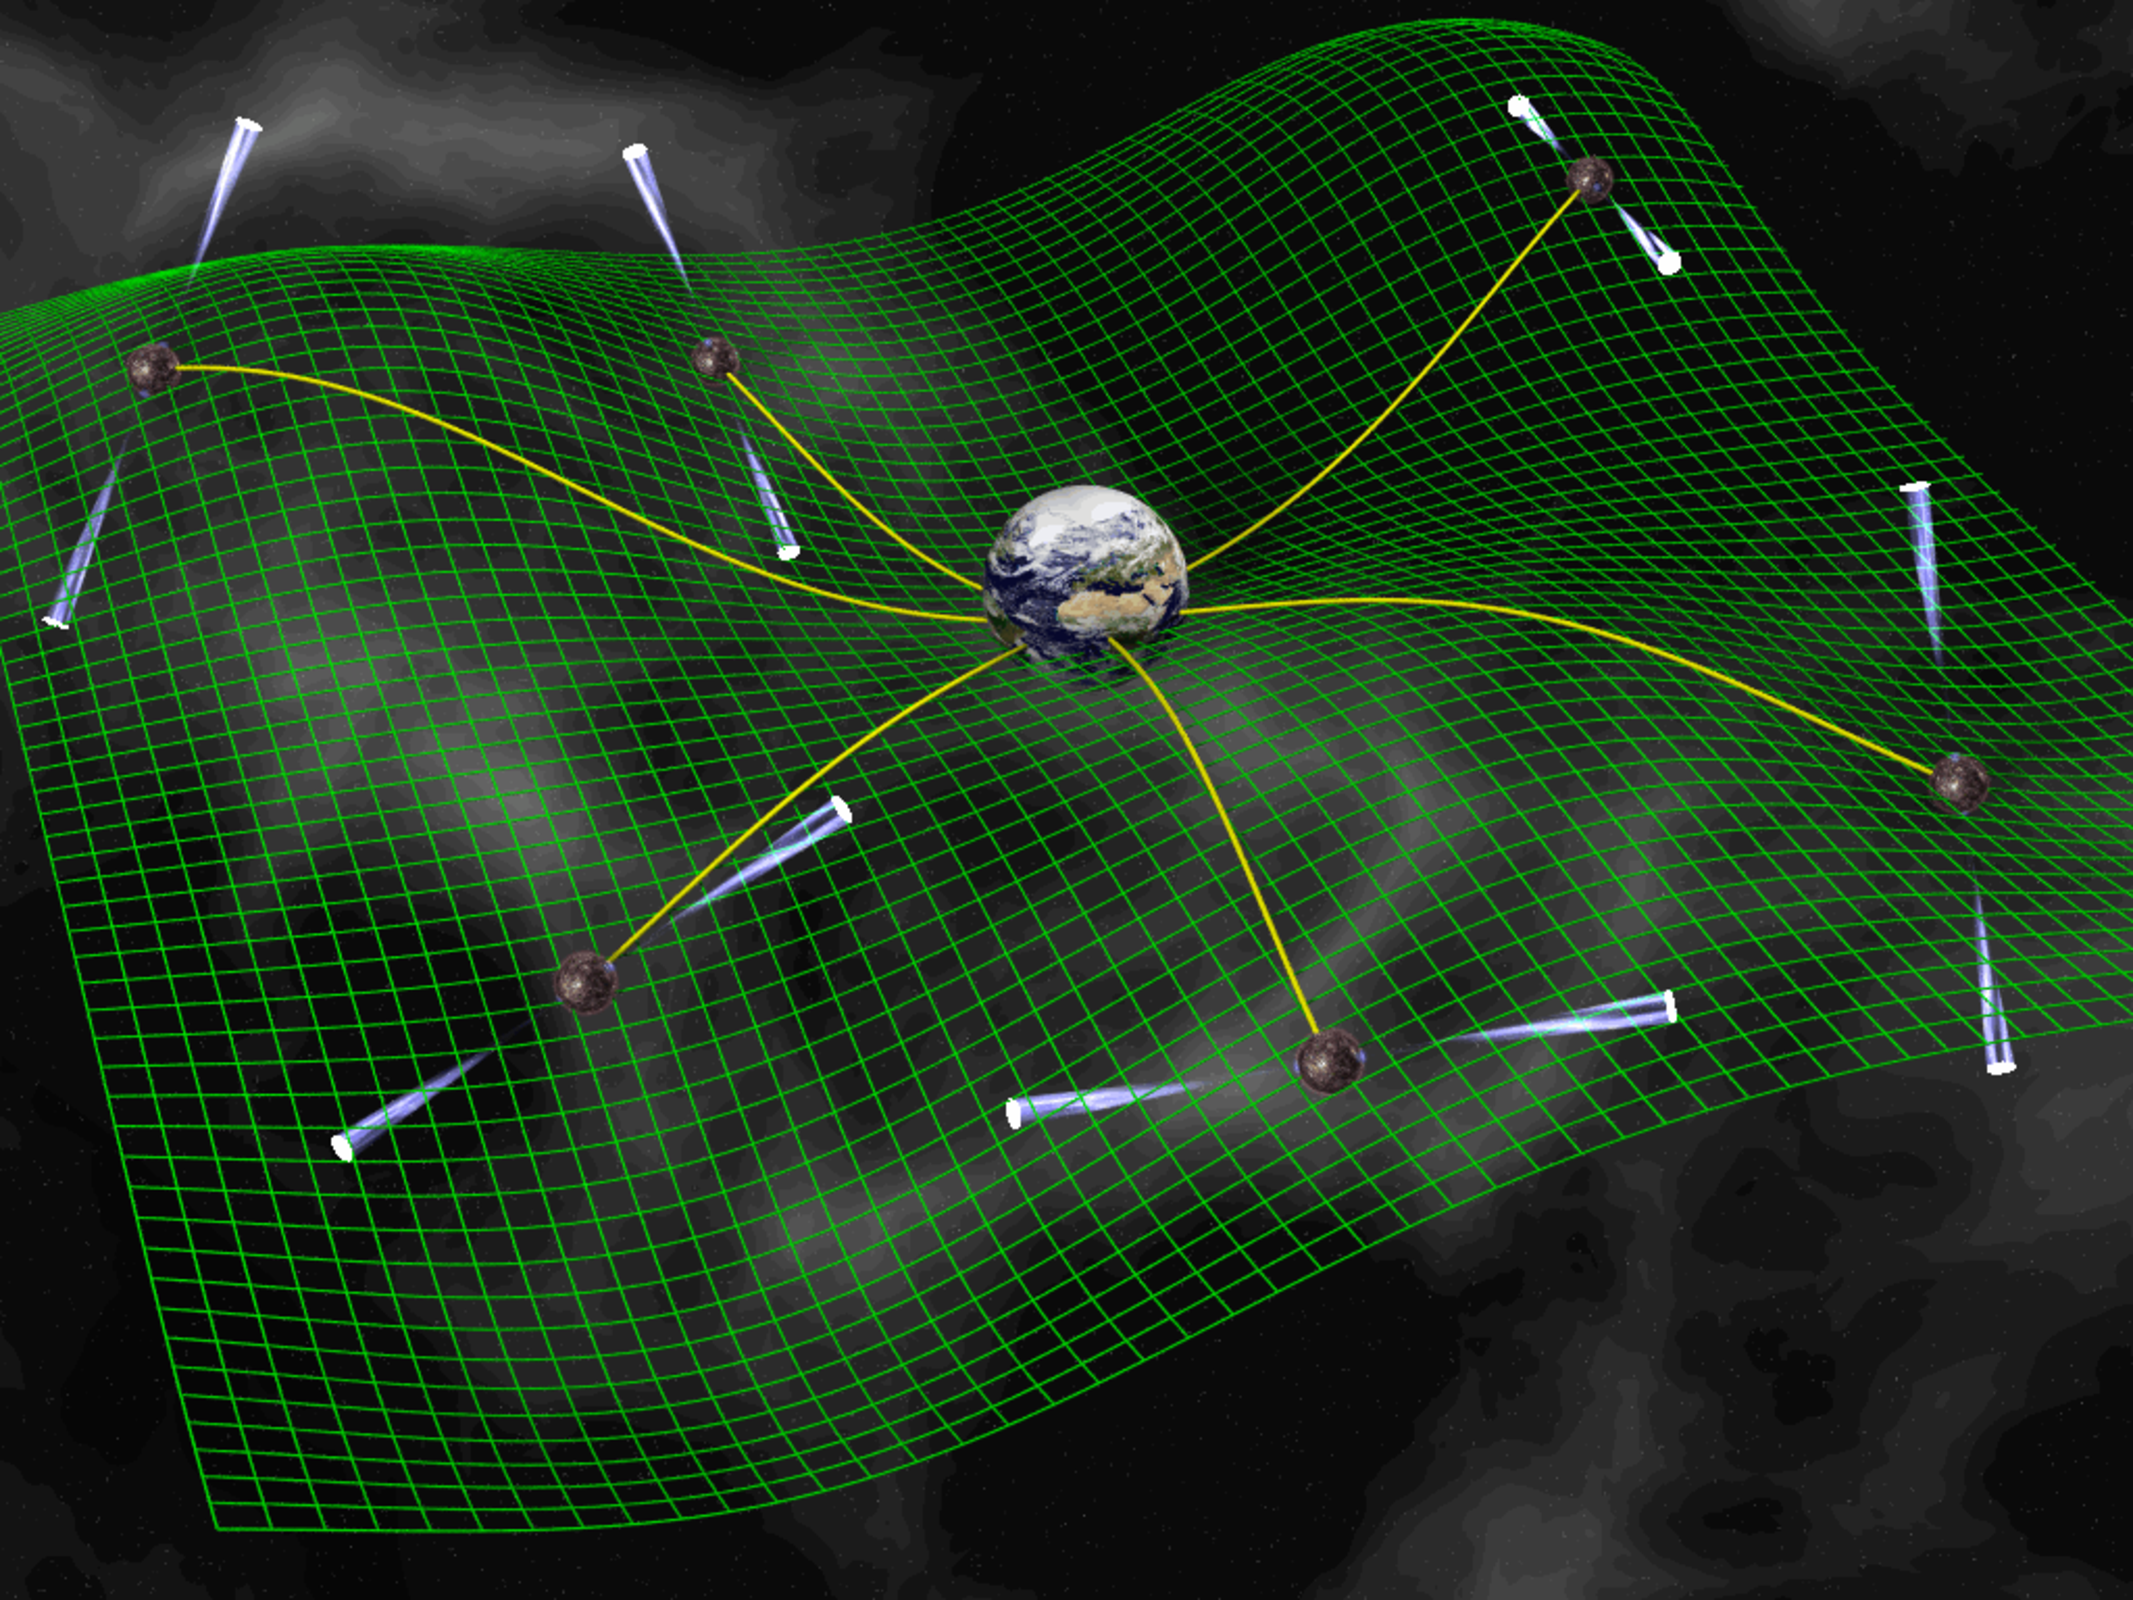
\includegraphics[width=0.8\textwidth]{pta.pdf}
\end{frame}

%%%%%%%%%%%%%%%%%%%%%%%%%%%%%%%%%%%%%%%%%%%%%%%%%%%%%%%%%%%%%%%%%%%%%%
\begin{frame}{}
    \begin{itemize}
        \item 脉冲星计时残差之间的关联为
        {\small
        \e
        \langle\tilde{r}_I^*(f)\tilde{r}_J(f')\rangle
        = \frac{H_0^2}{16 \pi^4} \delta(f-f') f^{-5}
        \Gamma_{IJ} \Omega_{\rm GW}(f) .
        \q}
        \item 关联函数$\Gamma_{IJ}$依赖于脉冲星$I$和脉冲星$J$之间的夹角$\zeta$
        {\small\[
        \Gamma_{IJ}=\frac{3}{2} \left[ \frac{1}{3} +
        \frac{1-\cos\zeta}{2}\left[ \ln\lp\frac{1-\cos\zeta_{IJ}}{2}\rp
        - \frac{1}{6} \right] \right] +\frac{1}{2}\delta_{IJ}.
        \]}
        \centering
        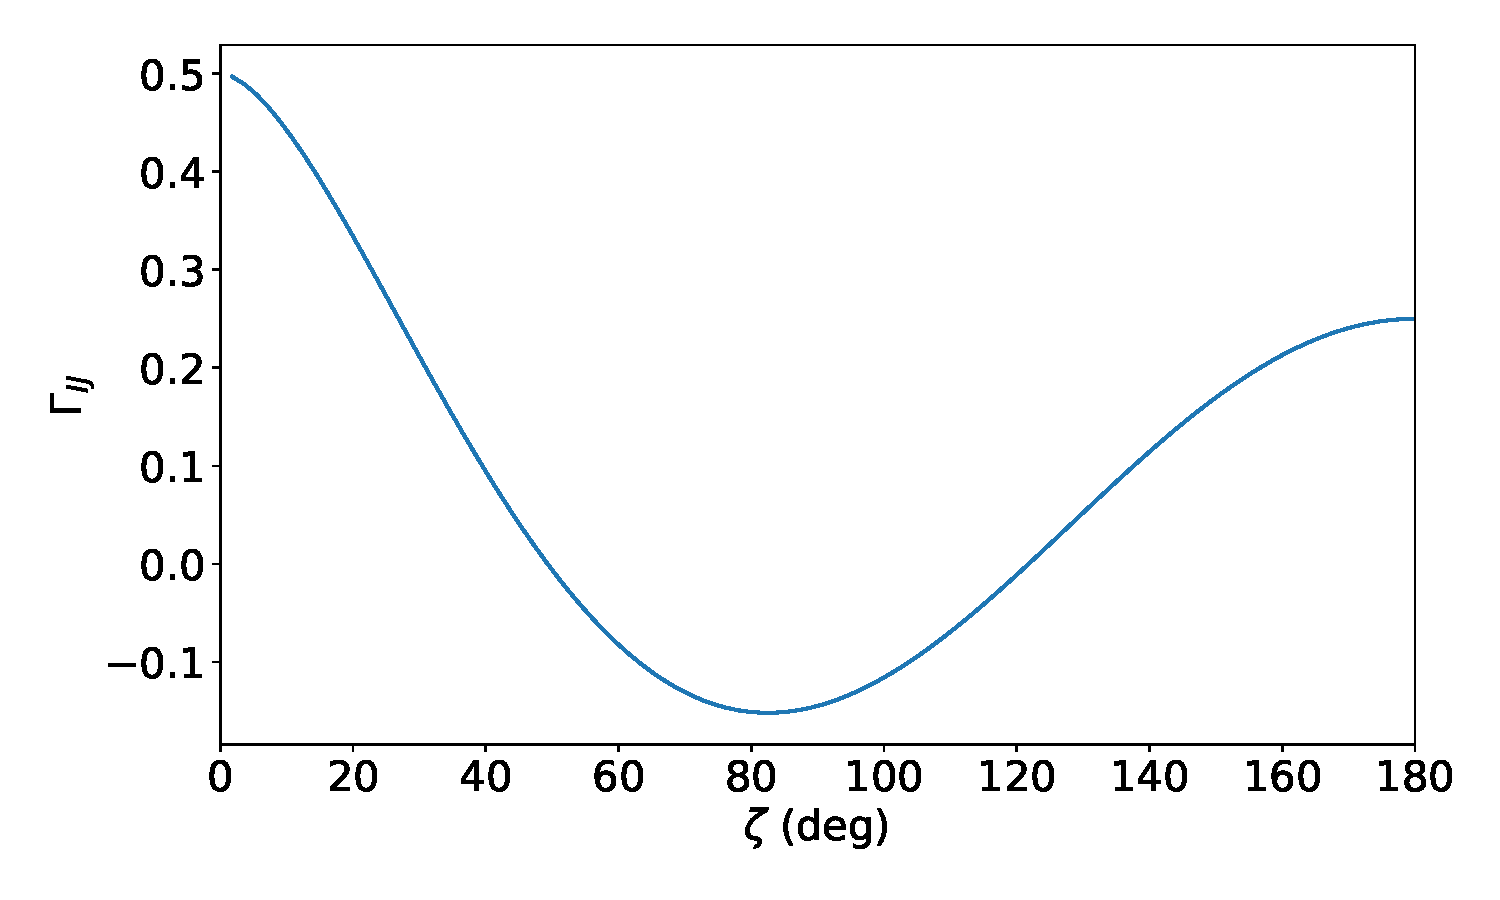
\includegraphics[width=0.8\textwidth]{Gamma.pdf}
    \end{itemize}
\end{frame}

%%%%%%%%%%%%%%%%%%%%%%%%%%%%%%%%%%%%%%%%%%%%%%%%%%%%%%%%%%%%%%%%%%%%%%
\begin{frame}{NANOGrav 11年的数据}
    \begin{table}[htb]
        \begin{center}
            \begin{tabular}{ccccc}
                \hline\hline
                脉冲星名称\hspace{1mm} & RMS [$\mu$s]\hspace{1mm} & $N_{\rm{epoch}}$\hspace{1mm} & $N_{\rm{TOA}}$\hspace{1mm} & $T_{\rm{obs}}$ [yr] \\
                \hline    
                J0613$-$0200 & 0.422 & 324 & 11,566 & 10.8  \\
                J1012$+$5307 & 1.07 & 493 & 16,782 & 11.4  \\
                J1600$-$3053 & 0.23 & 275 & 12,433 & 8.1  \\
                J1713$+$0747 & 0.108 & 789 & 27,571 & 10.9  \\
                J1744$-$1134 & 0.842 & 322 & 11,550 & 11.4  \\
                J1909$-$3744 & 0.148 & 451 & 17,373 & 11.2  \\    
                \hline \hline
            \end{tabular}
            \caption[数据分析中所使用的6颗脉冲星的基本属性:RMS--加权均方根计时残差,$N_{\rm{epoch}}$--观测数,$N_{\rm{TOA}}$--TOA数,$T_{\rm{obs}}$--观测时间跨度。]{数据分析中所使用的6颗脉冲星的基本属性:RMS--加权均方根计时残差,$N_{\rm{epoch}}$--观测数,$N_{\rm{TOA}}$--TOA数,$T_{\rm{obs}}$--观测时间跨度。}
                \end{center}
        \end{table}
\end{frame}


%%%%%%%%%%%%%%%%%%%%%%%%%%%%%%%%%%%%%%%%%%%%%%%%%%%%%%%%%%%%%%%%%%%%%%%
%\begin{frame}{数据分析}
%    \begin{itemize}
%        \item 从脉冲信号到达时间中扣除掉计时模型后的计时残差为
%        \e\label{noise}
%        \bn{} = \bn{RN} + \bn{WN} + \bn{SSE} + \bn{SIGW}.
%        \q 
%        \item $\bn{RN}$:红噪音
%        \item $\bn{WN}$:白噪音
%        \item $\bn{SSE}$:太阳系星历表修正
%        \item $\bn{SIGW}$:标量诱导引力波
%    \end{itemize}
%    
%\end{frame}


%%%%%%%%%%%%%%%%%%%%%%%%%%%%%%%%%%%%%%%%%%%%%%%%%%%%%%%%%%%%%%%%%%%%%%
\begin{frame}{曲率扰动功率谱的振幅$A$的上限}
    \begin{figure}[h!]
        \centering
        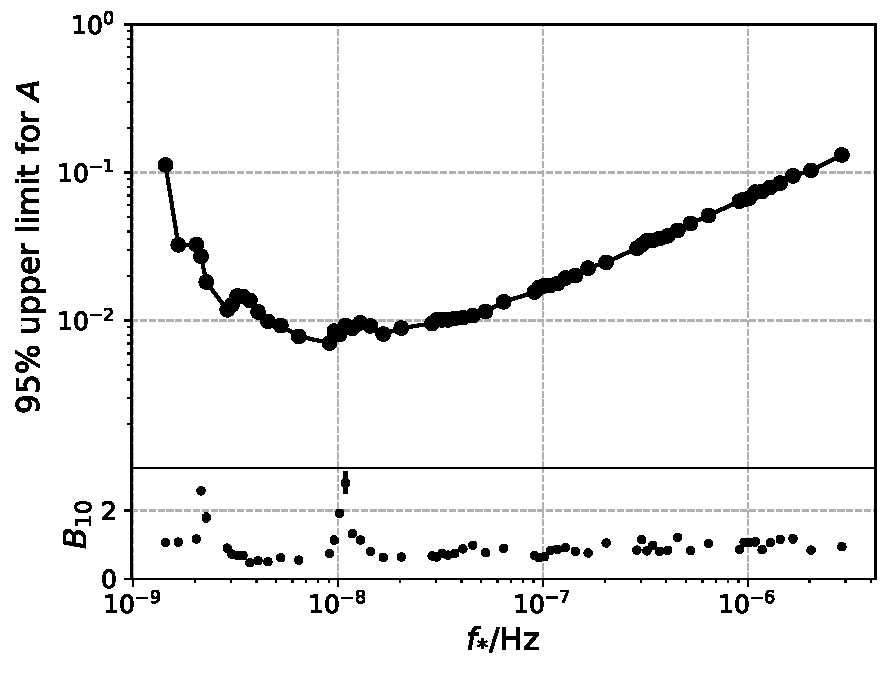
\includegraphics[width=0.7\textwidth]{A_upper.pdf}
        \caption{\label{A_upper} \textbf{上图}:曲率扰动功率谱振幅$A$的$95\%$上限与峰值频率$\fstar$的关系。\textbf{下图}:相应的贝叶斯因子$B_{10}$与峰值频率$\fstar$的关系。
        }
    \end{figure}
    
\end{frame}

%%%%%%%%%%%%%%%%%%%%%%%%%%%%%%%%%%%%%%%%%%%%%%%%%%%%%%%%%%%%%%%%%%%%%%
\begin{frame}{原初黑洞占冷暗物质丰度$\fpbh$的上限}
    \begin{figure}[h!]
        \centering
        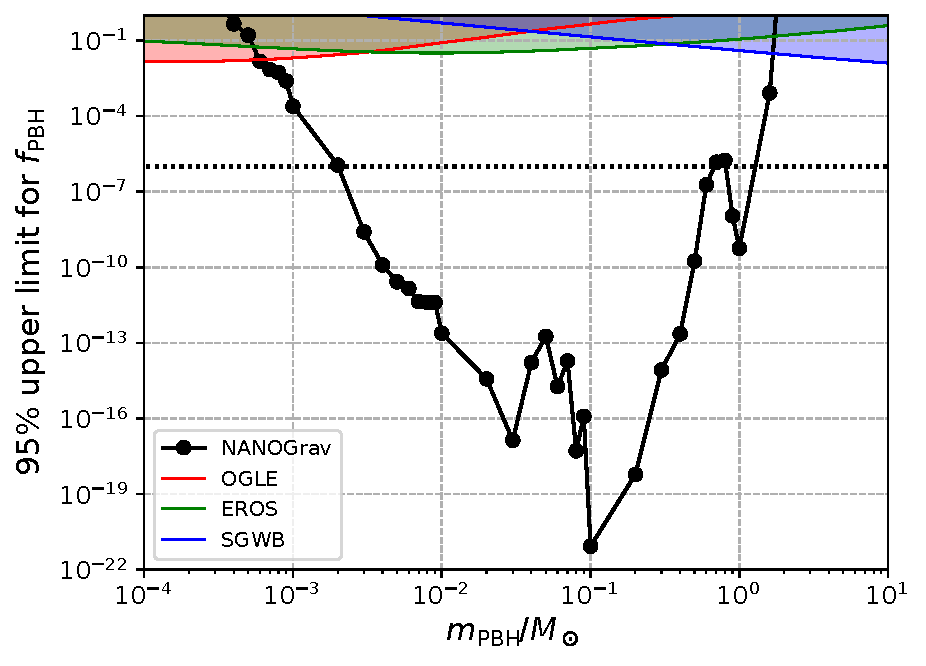
\includegraphics[width=0.7\textwidth]{fpbh_upper.pdf}
        \caption{\label{fpbh_upper} 原初黑洞占冷暗物质丰度$\fpbh$的$95\%$上限关于原初黑洞质量$m_{\rm{PBH}}$的函数。}
    \end{figure}    
\end{frame}

%%%%%%%%%%%%%%%%%%%%%%%%%%%%%%%%%%%%%%%%%%%%%%%%%%%%%%%%%%%%%%%%%%%%%%
\begin{frame}{小结}	
    \begin{itemize}        
        \item 计算了三阶标量诱导引力波。
        \item 在NANOGrav 11年的数据中搜索标量诱导引力波。由于没有发现引力波信号,对曲率扰动功率谱的振幅$A$和原初黑洞的丰度$\fpbh$给出上限。
        \item 在$0.002\sim 0.7\Msun$的质量区间,$\fpbh < 10^{-6}$。
    \end{itemize}
\end{frame}
%%%%%%%%%%%%%%%%%%%%%%%%%%%%%%%%%%%%%%%%%%%%%%%%%%%%%%%%%%%%%%%%%%%%%%

\section{总结}
%%%%%%%%%%%%%%%%%%%%%%%%%%%%%%%%%%%%%%%%%%%%%%%%%%%%%%%%%%%%%%%%%%%%%%
\begin{frame}{总结}
    \begin{itemize}
        \item 计算原初黑洞具有一般质量谱时,原初双黑洞的并合率分布;证实恒星级质量的原初黑洞无法构成绝大部分冷暗物质。
        
        \item 计算了原初双黑洞产生的随机引力波背景,并发现此背景可以被LISA探测到。如果此背景没能从LISA噪音中扣除掉,将会构成LISA的额外噪音,从而降低LISA的探测能力。
        
        \item 探讨如何通过ET和CE来区分原初黑洞和天体物理黑洞。通过定向搜寻包含至少一个亚太阳质量黑洞的双黑洞系统,估算了$\fpbh$的可探测极限。并预测了ET和CE能够探测到的双黑洞事件数目随红移的分布,从而来区分原初黑洞和天体物理黑洞。
        
        \item 在NANOGrav 11年的数据中搜寻伴随原初黑洞形成而产生的标量诱导引力波。由于没有发现引力波信号,所以在$0.002\sim 0.7\Msun$的质量区间,$\fpbh < 10^{-6}$。
    \end{itemize}  
\end{frame}

%%%%%%%%%%%%%%%%%%%%%%%%%%%%%%%%%%%%%%%%%%%%%%%%%%%%%%%%%%%%%%%%%%%%%%
\begin{frame}{展望}
    \begin{itemize}
        \item 用\lvc 最新的数据GWTC-2来重构原初黑洞质量谱$P(m)$以及拟合原初黑洞模型。
        
        \item 考虑原初黑洞和天体物理黑洞同时存在的情况。
        
        \item 在NANOGrav 12.5年的数据中搜索引力波信号:
        \begin{itemize}
            \item 标量诱导引力波
            \item 其它极化模式的引力波
        \end{itemize}
    \end{itemize}  
\end{frame}

%%%%%%%%%%%%%%%%%%%%%%%%%%%%%%%%%%%%%%%%%%%%%%%%%%%%%%%%%%%%%%%%%%%%%%
\begin{frame}[plain]
    \begin{center}
        \font\endfont = cmss20 at 25.40mm
        \color{Blue}
        \endfont
        \baselineskip 20.0mm
        \fontsize{50.0pt}{\baselineskip}\selectfont  谢谢!
    \end{center} 
\end{frame}
%%%%%%%%%%%%%%%%%%%%%%%%%%%%%%%%%%%%%%%%%%%%%%%%%%%%%%%%%%%%%%%%%%%%%%
%%%%%%%%%%%%%%%%%%%%%%%%%%%%%%%%%%%%%%%%%%%%%%%%%%%%%%%%%%%%%%%%%%%%%%
\end{document}
